\chapter{QUADRO METODOLÓGICO}

	\par Neste capítulo serão apresentados os métodos adotados para se realizar
	esta pesquisa, tais como: tipo de pesquisa, contexto, procedimentos, entre outros.
	
	%tipo de pesquisa
	\section{Tipo de pesquisa}
		\section{Tipo de pesquisa}
	
	\par Uma pesquisa é o ato de buscar e procurar pela resposta de algo.
\citeonline[p. 15]{markoni2002} definem pesquisa como “uma indagação minuciosa
ou exame crítico e exaustivo na procura de fatos e princípios”.

	\par Existem diversos tipos de pesquisa, no entanto percebeu-se que para o
propósito desta, a mais indicada foi a pesquisa aplicada, pois está se
desenvolvendo um projeto real que poderá ser utilizado por qualquer instituição
de ensino, mas que não mudará a forma com que as pessoas recebam suas
informações, apenas acrescentará mais uma opção de consultá-las.

	\par Segundo \citeonline[p. 15]{markoni2002}, uma pesquisa do tipo aplicada
“caracteriza-se por seu interesse prático, isto é, que os resultados sejam
aplicados ou utilizados, imediatamente, na solução de problemas que ocorrem na
realidade”.

	\par Dessa maneira, percebeu-se que esta pesquisa enquadra-se no tipo de pesquisa
aplicada, pois com a execução da mesma resolve um problema específico, e para
isso está desenvolvendo-se um aplicativo para dispositivos móveis que facilitará aos
graduandos acessarem o sistema \textit{web} de uma universidade.
	
	%contexto de pesquisa
	\section{Contexto de pesquisa}
		%\section{Contexto de pesquisa}

	\par Para que os alunos possam saber suas notas, faltas e provas agendadas,
é necessário que eles acessem o portal do aluno para consultá-las.

	\par O \textit{web service}, criado através desta pesquisa, tem por objetivo
fornecer a estrutura para que a Univás possa disponibilizar suas informações
através de serviços, bem como desenvolver um serviço para que o aplicativo
consulte as notas, faltas e provas agendadas dos alunos.

	\par A aplicação Android, por sua vez, tem por finalidade facilitar aos
estudantes o acesso às suas informações escolares mais procuradas.
	
	\par Os alunos acessarão o aplicativo com o mesmo usuário e senha do
portal do aluno, e quando houver o lançamento de alguma nota ou prova agendada,
eles serão notificados em seu dispositivo. Ao clicar na notificação
o sistema apresentará a informação recebida. 
	
	%instrumentos
	\section{Instrumentos}
		%\section{Instrumentos}

	\par Os instrumentos de pesquisa existem para que se possam levantar
informações para realizar um determinado projeto.

	\par Pode-se dizer que um questionário é uma forma de coletar
informações através de algumas perguntas feitas a um público específico.
Segundo \citeonline{gunther2003}, o questionário pode ser definido como
um conjunto de perguntas que mede a opinião e interesse do respondente.

	\par Neste trabalho foi realizado um questionário simples, apresentado na
Figura \ref{fig:qm1}, contendo quatro perguntas e enviado para \textit{e-mails}
de alguns alunos da universidade. O foco desse questionário era saber o motivo
pelo qual os usuários mais acessavam o portal do aluno e se tinham alguma
dificuldade em encontrar o que procuravam. Obteve-se um total de treze
respostas, no qual pode-se perceber que a maioria dos entrevistados afirmaram
ter dificuldades para encontrar as informações de que necessitam, e que
gostariam de ser notificados quando houvesse alguma atualização de notas. Sobre
o motivo do acesso, cem por cento dos discentes responderam que entram no
sistema \textit{web} para consultar os resultados das avaliações.

\begin{figure}[h!]
	\centerline{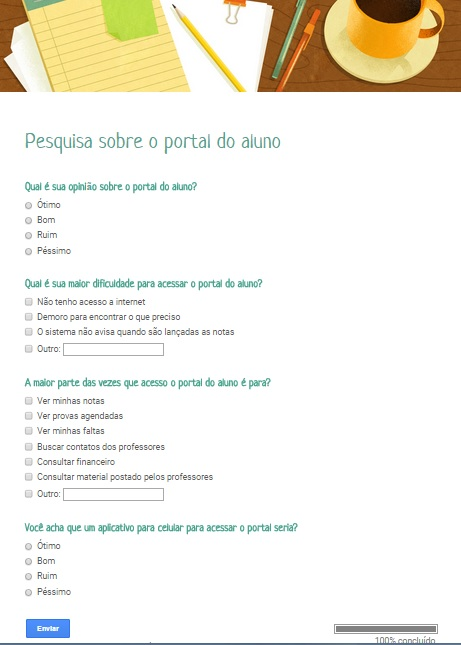
\includegraphics[scale=0.5]{./imagens/2_q_metodologico/qm1.png}}
	\caption[Quetionário Aplicado]{Quetionário Aplicado.
		\textbf{Fonte:}Elaborado pelos autores.}
	\label{fig:qm1}
\end{figure}
	

	\par Outro instrumento utilizado para realizar esta pesquisa foram as reuniões,
ou seja, reunir-se com uma ou mais pessoas em um local, físico ou remotamente
para tratar algum assunto específico. Para \citeonline{ferreira1999}, reunião é o ato de
encontro entre algumas pessoas em um determinado local, com finalidade de tratar
qualquer assunto.

	\par Durante a pesquisa, foram realizadas reuniões entre os participantes com
o objetivo de discutir o andamento das tarefas pela qual cada integrante responsabilizou-se
a fazer e traçar novas metas. Também foram utilizadas referências
de livros, revistas, manuais e \textit{web sites}.
	
	%Procedimentos e resultados
	\section{Procedimentos e Resultados}
		%\section{Procedimentos e Resultados}

	
			%Modelagem
			\subsection{Lenvantamento de Requisitos}
				%\subsection{Modelagem}
	\par Ao decidir-se por esta pesquisa foi preciso entender os pontos
necessários para o bom funcionamento do software. As soluções geradas por este
trabalho tendem a atender os seguintes requisitos:

	\begin{itemize}
		\item Disponibilidade: O \textit{web service} foi projetado para criar uma
		estrutura pela qual a universidade pudesse disponibilizar informações através
		de serviços. Por isso, o servidor não pode ficar impossibilitado de responder
		as requisições por causa de falhas no sistema desenvolvido.
		\item Simplicidade: Segundo as respostas obtidas através do questionário
		aplicado, os estudantes encontram dificuldades para encontrar o que procuram
		quando acessam o portal do aluno. Portanto, o aplicativo Android, deve possuir
		uma interface simples e objetiva para levar as informações aos usuários.
		\item Notificação: Geralmente, o aluno acessa várias vezes ao dia o portal do
		aluno para saber se foi postada sua nota. Pensando nisso, o software precisa
		avisá-lo através de uma notificação quando uma nova informação for lançada no
		portal do aluno e ao clicar nesta notificação, deve ser apresentado a ele os
		dados lançados.
		\item Velocidade: Os dispositivos móveis conseguem informações em tempo real.
		Também, estando ciente que as pessoas utilizam os dispositivos móveis para
		ganhar tempo, é indispensável que as informações cheguem ao aluno o mais breve
		possível.
	\end{itemize}

	\par Tendo estes paradigmas em mente, passou-se a desenvolver o software, como
pode ser acompanhado nas seções seguintes.

	
			%gcm
			\subsection{Google Cloud Messaging(GCM)}
				%\subsection{\textit{Google Cloud Messaging}}

	\par O envio dos dados do \textit{web service} para o aplicativo
\textit{Android}, é feito através de um serviço da \textit{Google} conhecido
como GCM.

	\par Para que o serviço apresente o resultado esperado, foi preciso acessar o
\textit{site} da \textit{Google Developers Console} e criar um novo projeto. Ao
criá-lo, foi necessário ir na aba API's e ativar a opção \textit{Google Cloud
Messaging for Android}.

 	\par Com a criação do projeto, a \textit{Google} oferece um número que
identificará o \textit{software}, também chamado de \texttt{Sender ID},
conforme mostra a Figura \ref{fig:gcm}.


	\begin{figure}[h!] 
		\centerline{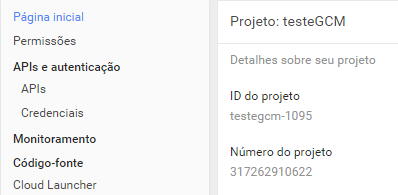
\includegraphics[scale=1]{./imagens/2_q_metodologico/4_procedimentos_resultados/41_gcm/gcm.png}}
		\caption[\texttt{Sender ID} do GCM]{\texttt{Sender ID} do GCM.
		\textbf{Fonte:}Elaborado pelos autores.}
		\label{fig:gcm}
	\end{figure}
	\pagebreak
	
	\par Por fim, acessou-se a aba Credenciais para indicar o IP do servidor. Ao
informa-lo, o serviço gerou uma chave pública a qual foi inserida no
\textit{web service}. Na Figura \ref{fig:gcm1}, é possível ver o código de
acesso criado.


	\begin{figure}[h!] 
		\centerline{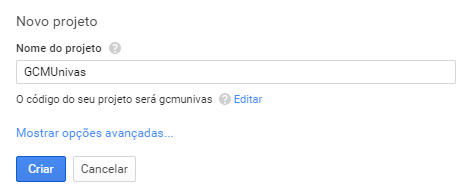
\includegraphics[scale=0.5]{./imagens/2_q_metodologico/4_procedimentos_resultados/41_gcm/gcm1.png}}
		\caption[Geração da credencial do GCM]{Geração da credencial do GCM.
		\textbf{Fonte:}Elaborado pelos autores.}
		\label{fig:gcm1}
	\end{figure}
	
			%Aplicativo
			\subsection{Aplicativo}
				%\subsection{Aplicativo}

	\par O primeiro passo realizado para a construção do aplicativo Android, foi a
modelagem do software através dos diagramas de UML, que permitiram nortear o
desenvolvimento.

	\par A princípio projetou-se um diagrama para se ter uma visão geral do
aplicativo. Nele pode-se ver a arquitetura da aplicação, bem como a comunicação
com o GCM e o \textit{web service}.

	\par Quando o servidor precisa enviar uma informação para os dispositivos
móveis, ele envia a mensagem ao GCM, que a transfere para aplicativo. Ao
receber os dados, a classe \texttt{GcmBroadcastReceiverUnivas} executa a classe
\texttt{GcmIntentServiceUnivas} que por sua vez irá notificar o usuário,
contudo antes de notificá-lo, ela envia as informações para a classe
\texttt{HttpUtil}, que faz a conversão dos dados vindos em JSON para o formato
da classe \texttt{EventTO}. Ao finalizar a leitura e conversão dos elementos,
as informações são enviadas para a classe \texttt{DatabaseExecute} que realiza
a gravação dos dados no banco de dados.

	\par Quando o usuário clica na notificação, é apresentada a ele uma
\textit{activity} a qual exibe as informações recebidas. Neste contexto, quando
o evento recebido se tratar de uma nota será aberta a \textit{activity}
\texttt{NotificationResultsActivity}, no caso de ser uma falta é executada a
\textit{activity} \texttt{NotificationFoulsActivity} e caso for um evento de
provas agendadas então é mostrada a \textit{activity}
\texttt{NotificationAgendasActivity}.

	\par Para o estudante visualizar suas informações, ele acessará a classe
\texttt{MainActivity}. Se desejar ver as suas notas, então é apresentada a
\textit{activity} \texttt{ListResultsActivity}, que utiliza a classe
\texttt{ListResultsAdapter} para gerenciar as informações e apresentá-las ao
discente. No entanto, se escolher a opção de faltas, é apresentada a
\textit{activity} \texttt{ListFoulsActivity}, que receberá as informações da
classe \texttt{ListFoulsAdapter} e caso decida-se pela opção provas agendadas é
exibida a \textit{activity} \texttt{ListAgendasActivity}, gerenciada pela
classe \texttt{ListAgendasAdapter}.

	\par A classe \texttt{GcmControllerUnivas}, tem por finalidade cadastrar o
dispositivo no GCM e enviar a chave gerada para o \textit{web service}. Na
Figura \ref{fig:app}, é apresentado o diagrama de arquitetura.

	\begin{figure}[h!] 
		\centerline{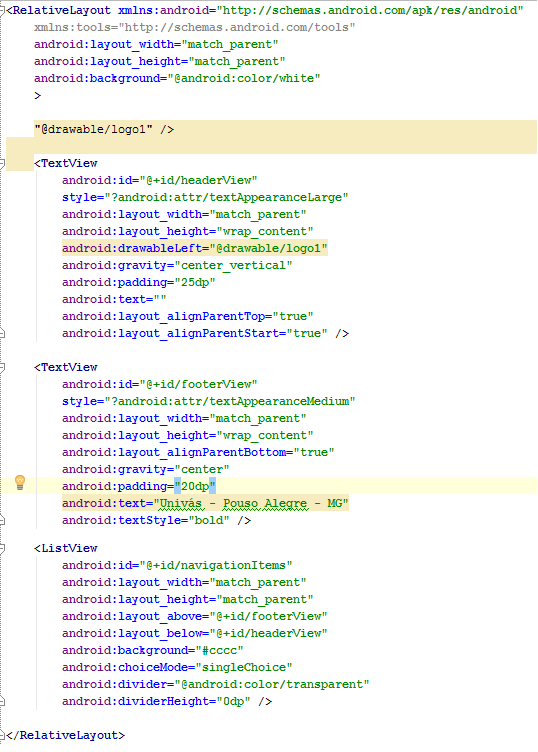
\includegraphics[scale=0.42]{./imagens/2_q_metodologico/4_procedimentos_resultados/42_aplicativo/app.png}}
		\caption[Diagrama de arquitetura do aplicativo]{Diagrama de arquitetura do aplicativo.
		\textbf{Fonte:}Elaborado pelos autores.}
		\label{fig:app}
	\end{figure}
	
	\par Posteriormente, foi desenvolvido o diagrama de caso de usos, com
finalidade em ter uma visão das funcionalidades do software pelo lado do
usuário. O utilitário permite ao aluno receber notificações quando for lançada
uma nova nota, falta ou prova agendada e visualizar estas informações. Na
Figura \ref{fig:app1} é possível ver o diagrama de casos de uso.

	\begin{figure}[h!] 
		\centerline{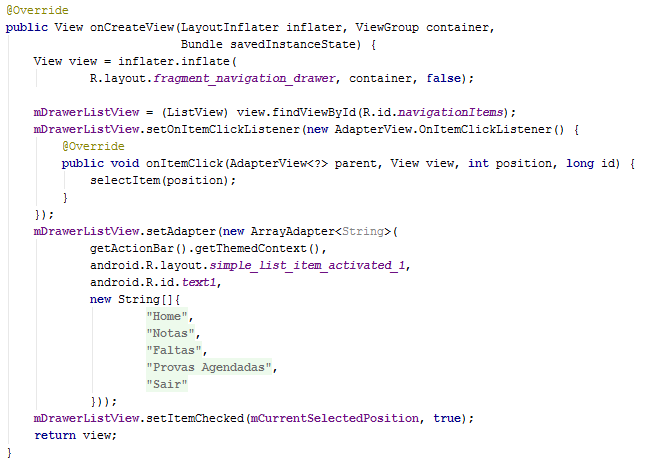
\includegraphics[scale=0.7]{./imagens/2_q_metodologico/4_procedimentos_resultados/42_aplicativo/app1.png}}
		\caption[Diagrama de casos de uso]{Diagrama de casos de uso.
		\textbf{Fonte:}Elaborado pelos autores.}
		\label{fig:app1}
	\end{figure}
	
	\par Para iniciar a construção do aplicativo, fez-se necessário a instalação e
configuração do ambiente de desenvolvimento. Primeiramente, realizou-se o
\textit{download} da IDE Android Studio, versão 1.1.0 e do Android SDK, versão
24.0.2, ambos no site \textit{Developers} Android através do endereço
\url{https://developer.android.com/intl/pt-br/sdk/index.html}.

	\par Contudo, ao executar o emulador do Android o sistema apresentava a
seguinte mensagem: “\textit{emulator: Failed to open the HAX device!}”. Depois
de algum tempo pesquisando, percebeu-se que era necessário instalar um programa
chamado Intel \textit{Hardware Accelerated Execution Manager} (HAXM), que
permite a execução do emulador Android mais rápido.

	\par No entanto, ao instalá-lo ocorria o seguinte erro: “\textit{this computer
meets the requirements for haxm but intel virtualization technology (VT-x) is
not turned on.}” A solução foi acessar a BIOS da máquina e habilitar o
assistente de hardware para virtualização. Daí em diante, foi possível executar
no emulador as aplicações feitas no Android Studio.

	\par Com o ambiente já configurado, houve a necessidade de se criar um
repositório no controlador de versão Github, o qual pode ser acessado através
do endereço \url{https://github.com/diegodnunes12/AppTCC} e compartilhado entre
os participantes do projeto.

	\par A partir de então, passou-se a desenvolver o software. A princípio, foi
construída uma \textit{activity}, que é acessível ao aluno logo que a aplicação
se inicia. Essa \textit{activity} é do tipo \textit{Navigation Drawer Layout},
ou seja, é um painel que permite inserir as opções de navegação do aplicativo,
semelhante a um menu.	Ao criar essa \textit{activity}, o Android Studio gera
automaticamente a classe \texttt{NavigationDrawerFragment} e um arquivo XML na
pasta \textit{layout}, chamado \texttt{fragment\_navigation\_drawer.xml}.

	\par No arquivo \texttt{fragment\_navigation\_drawer.xml} foram inseridos três
\textit{widgets}, sendo dois do tipo \texttt{textView}, para o cabeçalho com a
logomarca da Univás e para o rodapé com o seguinte texto: “Univás – Pouso
Alegre – MG” e um \textit{widget} do tipo \texttt{listView} que contém a lista
com as opções que o software oferece ao aluno.

	\par O \textit{layout} desta \textit{activity} chama-se
\textit{relativeLayout}, o qual permite um elemento ser posicionado em relação
a um outro. Desta forma o \textit{widget} \textit{listView} do Android, utiliza
a propriedade \texttt{android:layout\_below="@+id/headerView"} para se posicionar abaixo do
componente com id \textit{headerView} e a propriedade
\texttt{android:layout\_above="@+id/footerView"} indicando que ela deve preceder
o \textit{widget} com id \textit{footerView}. Na Figura \ref{fig:app2}, pode
ser visto o código XML dos \textit{widgets} desta tela.

	\begin{figure}[h!] 
		\begin{lstlisting}[style=custom_XML]
	<RelativeLayout xmlns:android="http://schemas.android.com/apk/res/android"
    xmlns:tools="http://schemas.android.com/tools"
    android:layout_width="match_parent"
    android:layout_height="match_parent"
    android:background="@android:color/white">
	    <TextView
	        android:id="@+id/headerView"
	        style="?android:attr/textAppearanceLarge"
	        android:layout_width="match_parent"
	        android:layout_height="wrap_content"
	        android:drawableLeft="@drawable/logo1"
	        android:gravity="center_vertical"
	        android:paddingTop="5dp"
	        android:paddingBottom="5dp"
	        android:paddingLeft="25dp"
	        android:paddingRight="25dp"
	        android:text=""
	        android:layout_alignParentTop="true"
	        android:layout_alignParentStart="true" />
	    <TextView
	        android:id="@+id/footerView"
	        style="?android:attr/textAppearanceMedium"
	        android:layout_width="match_parent"
	        android:layout_height="wrap_content"
	        android:layout_alignParentBottom="true"
	        android:gravity="center"
	        android:padding="20dp"
	        android:textColor="#228B22"
	        android:text="Univas - Pouso Alegre - MG"
	        android:textStyle="bold" />
	    <ListView
	        android:id="@+id/navigationItems"
	        android:layout_width="match_parent"
	        android:layout_height="match_parent"
	        android:layout_above="@+id/footerView"
	        android:layout_below="@+id/headerView"
	        android:background="#228B22"
	        android:choiceMode="singleChoice"
	        android:divider="@android:color/transparent"
	        android:dividerHeight="1dp" />
</RelativeLayout>
\end{lstlisting}
		\caption[Código dos widgets do arquivo
		fragment\_navigation\_drawer.xml]{Código dos \textit{widgets} do arquivo
		\texttt{fragment\_navigation\_drawer.xml}.
		\textbf{Fonte:}Elaborado pelos autores.}
		\label{fig:app2}
	\end{figure}
	
	\pagebreak
	
	\par A classe \texttt{NavigationDrawerFragment} representa o painel de
navegação. Nela se destaca o método \texttt{onCreateView()}, responsável por
criar o \textit{layout} de navegação. Na Figura \ref{fig:app3}, é mostrado o
método \texttt{onCreateView()} informando ao sistema operacional o \textit{layout} a
ser carregado e adicionando a um \textit{array} de \textit{String} as
alternativas de navegação que serão exibidos no \textit{listView} da tela
principal. Pode-se perceber também o método \texttt{onItemClick()}, que é
executado no momento em que o usuário clica em algum item da lista. 
	


	\begin{figure}[h!] 
		\begin{lstlisting}[style=custom_JAVA]
@Override
public View onCreateView(
		LayoutInflater inflater, ViewGroup container,Bundle savedInstanceState) {
    View view = inflater.inflate(
            R.layout.fragment_navigation_drawer, container, false);

    mDrawerListView = (ListView) view.findViewById(R.id.navigationItems);
    mDrawerListView.setOnItemClickListener(new AdapterView.OnItemClickListener() {
        @Override
        public void onItemClick(AdapterView<?> parent, View view, int position, long id) {
            selectItem(position);
        }
    });
    mDrawerListView.setAdapter(new ArrayAdapter<String>(
            getActionBar().getThemedContext(),
            android.R.layout.simple_list_item_activated_1,
            android.R.id.text1,
            new String[]{
                    getString(R.string.title_section1),
                    getString(R.string.title_section2),
                    getString(R.string.title_section3),
                    getString(R.string.title_section4),
                    getString(R.string.title_section5)
            }));
    mDrawerListView.setItemChecked(mCurrentSelectedPosition, true);
    return view;
}
public boolean isDrawerOpen() {
    return mDrawerLayout != null && mDrawerLayout.isDrawerOpen(mFragmentContainerView);
}
\end{lstlisting}
		\caption[Método onCreateView()]{Método \texttt{onCreateView()}.
		\textbf{Fonte:}Elaborado pelos autores.}
		\label{fig:app3}
	\end{figure}
	
	\pagebreak
	
	\par Nesse caso, quando for selecionada alguma opção da tela principal será
executado o método \texttt{selectItem()} apresentado na Figura \ref{fig:app4}, o
qual é responsável por retornar a posição do \textit{array} em que se encontra a
opção selecionada pelo aluno.
	
	\begin{figure}[h!] 
		\begin{lstlisting}[style=custom_JAVA]
	private void selectItem(int position) {
        mCurrentSelectedPosition = position;
        if (mDrawerListView != null) {
            mDrawerListView.setItemChecked(position, true);
        }
        if (mDrawerLayout != null) {
            mDrawerLayout.closeDrawer(mFragmentContainerView);
        }
        if (mCallbacks != null) {
            mCallbacks.onNavigationDrawerItemSelected(position);
        }
    }
\end{lstlisting}
		\caption[método selectItem()]{método \texttt{selectItem()}.
		\textbf{Fonte:}Elaborado pelos autores.}
		\label{fig:app4}
	\end{figure}
	
	\par O próximo passo foi criar o banco de dados do aplicativo para salvar as
informações recebidas do \textit{web service}. Para que isso fosse possível,
elaborou-se uma classe denominada \texttt{DatabaseHelper} que estende da classe
\texttt{SQLiteOpenHelper} do Android, com dois métodos, um chamado
\textit{onCreate()} que cria a estrutura do banco de dados e outro conhecido
por \textit{onUpgrade()}, usado se for necessário atualizar a estrutura do
banco de dados.

	\par Foi preciso criar um atributo que mantém a versão do banco de dados. Essa
informação serve para que o Android consiga saber qual dos dois métodos devem
ser executados. Ao iniciar a aplicação pela primeira vez, estando a versão em 1
(um), o sistema chamará o método \texttt{onCreate()}. Se for preciso atualizar
a estrutura do banco, o atributo versão deve ser incrementado em 1 (um), de
modo que ao executar o software o sistema operacional perceba a mudança,
chamando o método \texttt{onUpgrade()}. Na Figura \ref{fig:app5} é apresentado a
classe \texttt{DatabaseHelper}.

	\begin{figure}[h!] 
		\begin{lstlisting}[style=custom_JAVA]
public class DatabaseHelper extends SQLiteOpenHelper {

    private static final String BANCO_DADOS = "univasDB";
    private static int VERSAO = 1;

    public DatabaseHelper(Context context) {
        super(context, BANCO_DADOS, null, VERSAO);
    }
    @Override
    public void onCreate(SQLiteDatabase db) {
        db.execSQL("CREATE TABLE disciplinas (_id LONG PRIMARY KEY, nome TEXT);");

        db.execSQL("CREATE TABLE eventos (_id LONG PRIMARY KEY, id_disciplina LONG, " +
                " tipo_evento TEXT, descricao_evento TEXT," +
                " data_evento TEXT, valor_evento INTEGER, nota INTEGER,"  +
                " FOREIGN KEY (id_disciplina) REFERENCES disciplinas (_id) );");
    }
    @Override
    public void onUpgrade(SQLiteDatabase db, int i, int i2) {
        //Nao ha atuaizacoes no momento
    }
}
\end{lstlisting}
		\caption[Classe DatabaseHelper]{Classe \texttt{DatabaseHelper}.
		\textbf{Fonte:}Elaborado pelos autores.}
		\label{fig:app5}
	\end{figure}
	
	\par Em seguida foi criada a classe responsável por executar as consultas SQL,
denominada \texttt{DatabaseExecute}. Nela foram inseridos os métodos
responsáveis por inserir, alterar e buscar os dados dos alunos no banco de
dados local do aplicativo. Na Figura \ref{fig:app6}, pode-se observar o método
que possibilita a inserção dos eventos ocorridos. Esses eventos podem ser
notas, faltas ou provas agendadas.
	
	
	\begin{figure}[h!] 
		\begin{lstlisting}[style=custom_JAVA]
public void insertEvents(EventTO to){
        SQLiteDatabase db = helper.getWritableDatabase();

        ContentValues values = new ContentValues();
        values.put("_id", to.get_id());
        values.put("id_disciplina", to.getId_discipline());
        values.put("tipo_evento", to.getType_event());
        values.put("descricao_evento", to.getDescription_event());
        values.put("data_evento", to.getDate_event());
        values.put("valor_evento", to.getValue_event());
        values.put("nota", to.getResult());

        long result = db.insert("eventos", null, values);

        if(result != -1 ){
            Log.d(TAG, " Evento salvo com sucesso!");
        }else{
            Log.d(TAG, " Erro ao salvar o Evento!");
        }
    }
\end{lstlisting}
		\caption[Método de inserção de eventos]{Método de inserção de eventos.
		\textbf{Fonte:}Elaborado pelos autores.}
		\label{fig:app6}
	\end{figure}
	
	\pagebreak
	
	\par Este método recebe um objeto da classe \texttt{EventTO} com os elementos
necessários para inserir o evento no banco de dados. Para que seja possível a
inserção dos dados, \citeonline{monteiro2012}, afirma que é necessário
recuperar a referência da classe \texttt{SQLiteDatabase} através do método
\texttt{getWritableDatabase()}, logo após é instanciada a classe
\texttt{ContentValues}, onde são informados os campos da tabela e os
respectivos valores. Ao concluir, é chamado o \texttt{insert()} da classe
\texttt{SQLiteDatabase} informando o nome da tabela e o objeto da classe
\texttt{ContentValues}.

	\par Para listar os resultados dos exames realizados pelos discentes no painel
de notas é utilizado o método \texttt{getResults()} que retorna uma lista de
objetos da classe \texttt{EventTO}. De acordo com \citeonline{monteiro2012},
para conseguir recuperar as informações armazenadas no banco de dados é preciso
adquirir a instância de leitura da classe \texttt{SQLiteDatabase} através do
método \texttt{getReadableDatabase()}. Por meio dele pode-se realizar a
consulta, que devolve um \textit{Cursor} para navegar pelos resultados. Por
fim, é composto um objeto do tipo \texttt{EventTO} e inserido na lista. Na
Figura \ref{fig:app7} é apresentado o método \texttt{getResults()}.

	\par Foram inseridos mais dois métodos semelhantes ao \texttt{getResults()},
que são os métodos de \texttt{getFouls()} e \texttt{getAgendas()} para
recuperar as faltas e provas agendadas respectivamente. O que diferencia-os é a
consulta SQL, já que no \texttt{getFouls()}  foram buscados os dados onde o
\texttt{tipo\_evento = ‘FALTAS'} e no \texttt{getAgendas()} onde o
\texttt{tipo\_evento = ‘PROVA\_AGENDADA'}.

	\begin{figure}[h!] 
		\begin{lstlisting}[style=custom_JAVA]
public List<EventTO> getResults(){
        List<EventTO> notasTO = new ArrayList<>();

        SQLiteDatabase db = helper.getReadableDatabase();
        Cursor cursor =
                db.rawQuery("SELECT _id, id_disciplina, descricao_evento, valor_evento, nota  FROM" +
                                " eventos WHERE tipo_evento = 'PROVA_APLICADA'",
                        null);
        cursor.moveToFirst();

        for(int i = 0; i<cursor.getCount();i++){
            EventTO nota = new EventTO();

            nota.set_id(cursor.getLong(0));
            nota.setId_discipline(cursor.getLong(1));
            nota.setDescription_event(cursor.getString(2));
            nota.setValue_event(cursor.getInt(3));
            nota.setResult(cursor.getInt(4));

            notasTO.add(nota);
            cursor.moveToNext();
        }
        cursor.close();
        return notasTO;
    }
\end{lstlisting}
		\caption[Método getResults()]{Método \texttt{getResults()}.
		\textbf{Fonte:}Elaborado pelos autores.}
		\label{fig:app7}
	\end{figure}
	
	\pagebreak
	
	\par A fim de estabelecer uma conexão entre o aplicativo e o \textit{web
service}, foi preciso conceder a permissão de acesso à internet no arquivo
\texttt{AndroidManifest.xml} da seguinte forma: \texttt{<uses-permission
android:name="android.permission.INTERNET" />}.

	\par Logo após, criou-se uma classe chamada de \texttt{HttpUtilUnivas} para ler
informações recebidas do \textit{web service}. Ela estende da classe
\texttt{AsyncTask} que executa a consulta em paralelo com a \textit{thread
main}, evitando travar a aplicação enquanto recebe as informações vindas do
\textit{web service}. Estes dados estão em formato JSON e foi utilizada a
biblioteca GSON para convertê-las para o formato da classe \texttt{EventTO}.
Após a leitura, o objeto da classe \texttt{EventTO} é enviado para a classe
\texttt{DatabaseExecute}, a fim de realizar a inserção os dados no banco. A
Figura \ref{fig:app8}, mostra a classe \texttt{HttpUtilUnivas}.

	\begin{figure}[h!] 
		\begin{lstlisting}[style=custom_JAVA]
try{
        HttpClient httpClient = new DefaultHttpClient();
        HttpGet request = new HttpGet();
        request.setURI(new URI(urlEvents));

        HttpResponse response = null;
        try {
            response = httpClient.execute(request);
        } catch (IOException e) {
            e.printStackTrace();
        }
        InputStream content = null;
        try {
            content = response.getEntity().getContent();
        } catch (IOException e) {
            e.printStackTrace();
        }
        Reader reader = new InputStreamReader(content);
        Gson gson = new Gson();
        returnEvents = gson.fromJson(reader, Events.class);

        for (int i = 0; i< returnEvents.getEventos().size(); i++){
            DatabaseExecute execute = new DatabaseExecute(helper);
            EventTO to = new EventTO();
            to.set_id((long) returnEvents.getEventos().get(i).getId_evento());
            to.setValue_event(returnEvents.getEventos().get(i).getValor());
            to.setDescription_event(returnEvents.getEventos().get(i).getDescricao());
            to.setId_discipline(returnEvents.getEventos().get(i).getId_disciplina());
            to.setDate_event(returnEvents.getEventos().get(i).getData());
            to.setResult(returnEvents.getEventos().get(i).getNota());
            to.setType_event(returnEvents.getEventos().get(i).getTipoEvento());

            if(execute.existingEvent(to.get_id()) == false){
                execute.insertEvents(to);
            }else{
                execute.updateEvent(to);
            }
        }
        content.close();
    } catch (URISyntaxException e) {
        e.printStackTrace();
    } catch (IOException e) {
        e.printStackTrace();
    }
\end{lstlisting}
		\caption[Código da classe HttpUtilUnivas que faz a leitura dos
		eventos]{Código da classe \texttt{HttpUtilUnivas} que faz a leitura dos
		eventos.
		\textbf{Fonte:}Elaborado pelos autores.}
		\label{fig:app8}
	\end{figure}
	
	\pagebreak
	
	\par Para usufruir da biblioteca GSON, foi fundamental adicioná-la como uma
dependência do projeto. Para isso, foi preciso ir ao Menu do Android Studio,
clicando em \textbf{File} e depois em \textbf{Project Structure}. Com a janela
da estrutura do projeto aberta, foi selecionada a aba \textbf{Dependencies} e
depois foi escolhido o ícone de mais \textbf{(+)} para adicionar novas
dependências, conforme mostra a Figura \ref{fig:app9}.
	
	\begin{figure}[h!] 
		\centerline{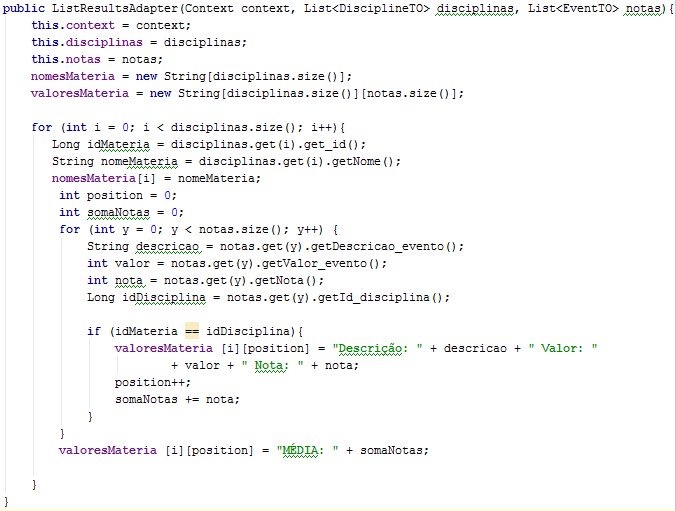
\includegraphics[scale=0.7]{./imagens/2_q_metodologico/4_procedimentos_resultados/42_aplicativo/app8.png}}
		\caption[Adicionando uma dependência ao projeto]{Adicionando uma dependência ao projeto.
		\textbf{Fonte:}Elaborado pelos autores.}
		\label{fig:app9}
	\end{figure}
	
	\par Na tela em que foi aberta localizou-se a biblioteca GSON com o endereço da
Google, logo após selecionou-a e clicou no botão Ok para adicioná-la, como
apresenta a Figura \ref{fig:app10}.
	
	\begin{figure}[h!] 
		\centerline{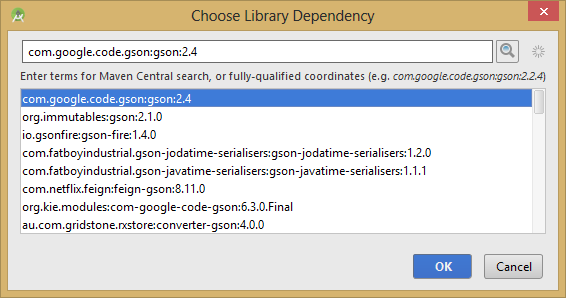
\includegraphics[scale=0.7]{./imagens/2_q_metodologico/4_procedimentos_resultados/42_aplicativo/app9.png}}
		\caption[Adicionando a biblioteca GSON ao projeto]{Adicionando a biblioteca GSON ao projeto.
		\textbf{Fonte:}Elaborado pelos autores.}
		\label{fig:app10}
	\end{figure}
	
	\par Na Figura \ref{fig:app11}, é mostrado o código onde é utilizado a
	biblioteca GSON. O sistema lê os dados vindos em JSON e envia para o GSON que faz a conversão dos
dados no formato da classe \texttt{EventTO}.

	\begin{figure}[h!] 
		\begin{lstlisting}[style=custom_JAVA]
			...
	Reader reader = new InputStreamReader(content);
    Gson gson = new Gson();
    retornoEventos = gson.fromJson(reader, Events.class);
			...
\end{lstlisting}
		\caption[Usando GSON para conversão dos dados]{Usando GSON para conversão dos dados.
		\textbf{Fonte:}Elaborado pelos autores.}
		\label{fig:app11}
	\end{figure}
	
	\par Depois, fez-se necessário construir uma classe que fizesse o gerenciamento
dos dados vindos do banco de dados com a interface que listará as informações
aos usuários. Essa classe recebeu o nome de \texttt{ListResultsAdapter} e
estende da classe nativa do Android denominada
\texttt{BaseExpandableListAdapter}.

	\par Nesta classe foi criado um construtor que recebe a lista de disciplinas
cursadas pelo aluno e uma lista com as notas de cada matéria. Os nomes das
disciplinas foram inseridos em um \textit{array} de \textit{Strings}, já as
notas foram inseridas em uma matriz. Este procedimento foi necessário devido a
estrutura dos métodos \texttt{getGroupView()} e \texttt{getChildView()}
responsável por apresentar na tela do dispositivo os nomes das disciplinas e as
notas das matérias respectivamente.  A Figura \ref{fig:app12} apresenta o
construtor da classe \texttt{ListResultsAdapter}.

	\begin{figure}[h!] 
		\begin{lstlisting}[style=custom_JAVA]
public ListResultsAdapter(Context context, List<DisciplineTO> disciplines, List<EventTO> results){
    this.context = context;
    this.disciplines = disciplines;
    this.results = results;
    namesDisciplines = new String[disciplines.size()];
    EventsDisciplines = new String[disciplines.size()][results.size()];

    for (int i = 0; i < disciplines.size(); i++){
        Long idDiscipline = disciplines.get(i).get_id();
        String nameDiscipline = disciplines.get(i).getName();
        namesDisciplines[i] = nameDiscipline;
        int position = 0;
        int totalResults = 0;
        for (int y = 0; y < results.size(); y++) {
            String description = results.get(y).getDescription_event();
            int value = results.get(y).getValue_event();
            int result = results.get(y).getResult();
            Long disciplineId = results.get(y).getId_discipline();

            if (idDiscipline == disciplineId){
                EventsDisciplines [i][position] = "Descricao: " + description +
                " Valor: " + value + " Nota: " + result;
                position++;
                totalResults += result;
            }
        }
        EventsDisciplines [i][position] = "SOMA DAS NOTAS: " + totalResults;
    }
}
\end{lstlisting}
		\caption[Construtor da classe ListResultsAdapter]{Construtor da classe ListResultsAdapter.
		\textbf{Fonte:}Elaborado pelos autores.}
		\label{fig:app12}
	\end{figure}

	\par Após adicionado os dados no \textit{array} e na matriz é preciso exibí-los
ao estudante. Na Figura \ref{fig:app13}, pode se ver o método \texttt{getGroupView()}
criando um \textit{widget} do tipo \textit{textView}  e inserindo nele o nome
da matéria, os espaçamentos, o tamanho da fonte e informando que as palavras
serão escritos em negrito.

	\begin{figure}[h!] 
		\begin{lstlisting}[style=custom_JAVA]
@Override
    public View getGroupView(int groupPosition, boolean isExpanded,
                             View convertView, ViewGroup parent) {

        TextView textViewDiscipline = new TextView(context);
        textViewDiscipline.setText(namesDisciplines[groupPosition]);
        textViewDiscipline.setPadding(40, 10, 0, 10);
        textViewDiscipline.setTextSize(20);
        textViewDiscipline.setTypeface(null, Typeface.BOLD);

        return textViewDiscipline;
    }
\end{lstlisting}
		\caption[Método getGroupView()]{Método \texttt{getGroupView()}.
		\textbf{Fonte:}Elaborado pelos autores.}
		\label{fig:app13}
	\end{figure}
	
	\pagebreak

	\par O método \texttt{getChildView()} segue a mesma lógica do método
\texttt{getGroupView()}, como ilustra a Fugura \ref{fig:app14}.

	\begin{figure}[h!] 
		\begin{lstlisting}[style=custom_JAVA]
@Override
    public View getChildView(int groupPosition, int childPosition,
                             boolean isLastChild, View convertView, ViewGroup parent) {

        TextView textViewSubList = new TextView(context);
        textViewSubList.setText(EventsDisciplines[groupPosition][childPosition]);
        textViewSubList.setPadding(10, 10, 10, 5);
        textViewSubList.setTextSize(15);

        return textViewSubList;
    }
\end{lstlisting}
		\caption[Método getChildView()]{Método \texttt{getChildView()}.
		\textbf{Fonte:}Elaborado pelos autores.}
		\label{fig:app14}
	\end{figure}
	
	\par O próximo passo, foi criação de uma \textit{activity} do tipo
\textit{blank activity} com finalidade de listar as notas. Ao criá-la com o
nome de \texttt{ListResultsActivity}, o Android Studio gerou dentro da pasta
\textit{layout} o arquivo XML referente a ela, chamado de
\texttt{activity\_list\_results.xml}. Neste, foi inserido apenas o
\textit{widget} \texttt{expandableListView}, que está incumbido de apresentar
a lista de disciplinas cujo o discente está cursando e ao clicar em alguma
dessas matérias serão apresentadas as notas referentes às atividades
realizadas nesta disciplina. Na Figura \ref{fig:app15} é possível ver o código XML de uma
lista do tipo \texttt{expandableListView}.

	\begin{figure}[h!] 
		\begin{lstlisting}[style=custom_XML]
<RelativeLayout 
	xmlns:android="http://schemas.android.com/apk/res/android"
    xmlns:tools="http://schemas.android.com/tools" 
    android:layout_width="match_parent"
    android:layout_height="match_parent" 
    android:paddingLeft="@dimen/activity_horizontal_margin"
    android:paddingRight="@dimen/activity_horizontal_margin"
    android:paddingTop="@dimen/activity_vertical_margin"
    android:paddingBottom="@dimen/activity_vertical_margin"
    android:theme="@style/AppTheme"
    tools:context="univas.edu.com.university.ListResultsActivity">

    <ExpandableListView
        android:layout_width="wrap_content"
        android:layout_height="wrap_content"
        android:id="@+id/expandableListView2"
        android:divider="#FFFFFF"
        android:dividerHeight="1dp"
        android:layout_alignParentBottom="true"
        android:layout_alignParentStart="true"
        android:layout_alignParentTop="true" />

</RelativeLayout>
\end{lstlisting}
		\caption[Código XML do layout que apresentará a lista de notas]{Código XML do
		\textit{layout} que apresentará a lista de notas.
		\textbf{Fonte:}Elaborado pelos autores.}
		\label{fig:app15}
	\end{figure}
	
	\pagebreak
	
	\par Na classe \texttt{ListResultsActivity}, é preciso informar o layout a ser
chamado através do método \texttt{setContentView()}. Além disso, também foi
necessário passar para a classe \texttt{ListResultsAdapter} a lista de
disciplinas que o discente está cursando e a lista com as notas referentes a
cada matéria vindas do banco de dados. Na Figura \ref{fig:app16} é exibido o
método \texttt{onCreate()} da classe \texttt{ListResultsActivity}. 
	
	
	\begin{figure}[h!] 
		\begin{lstlisting}[style=custom_JAVA]
@Override
protected void onCreate(Bundle savedInstanceState) {
    super.onCreate(savedInstanceState);
    setContentView(R.layout.activity_list_results);
    helper = new DatabaseHelper(this);

    execute = new DatabaseExecute(helper);

    ExpandableListView listView = 
    		(ExpandableListView) findViewById(R.id.expandableListView2);
    listView.setAdapter(
    	new ListResultsAdapter(
        	this, 
        	execute.getDisciplines(),
        	execute.getResults())
    	); 
}
\end{lstlisting}
		\caption[ Método onCreate() da classe ListResultsActivity]{ Método
		\texttt{onCreate()} da classe \texttt{ListResultsActivity}.
		\textbf{Fonte:}Elaborado pelos autores.}
		\label{fig:app16}
	\end{figure}

	\par Estes procedimentos que foram realizados para as classes
\texttt{ListResultsActivity} e \texttt{ListResultsAdapter}, eram necessários
para se apresentar as notas dos exercícios resolvidos. Desta mesma forma foi
preciso criar uma \textit{activity} e um \texttt{adapter} tanto para faltas
quanto para provas agendadas seguindo a mesma lógica.

	\par No momento em que algum professor lançar notas, faltas ou provas agendadas
no portal do aluno, é indispensável notificar o estudante. Com esse intuito
desenvolveu-se uma classe chamada de \texttt{GcmIntentServiceUnivas} que
estende \texttt{IntentService}, que recebe a mensagem vinda do GCM.

	\par Esta classe recebe os dados em formato JSON, por isso ela transfere estas
informações para o método \texttt{getJsonEvents()} da classe
\texttt{HttpUtilUnivas}, o qual será responsável por ler os dados e realizar os
procedimentos de gravação no banco de dados.

	\par Ao salvar o evento é chamado o método \texttt{sendNotification()}, que
receberá um objeto da classe \texttt{EventTO}. Ele realiza uma análise do tipo
de evento, para saber qual activity deve ser executada quando o usuário clicar
na notificação. Logo após adicionado os atributos da notificação, como o ícone,
o título e a mensagem, a notificação é exibida ao usuário. Na Figura
\ref{fig:app17} é visível o método \texttt{sendNotification()}.

	\begin{figure}[h!] 
		%\begin{lstlisting}[style=custom_JAVA]
private void sendNotification(EventTO to) {
        String msg;
        DisciplineTO disciplineTO = execute.getDispline(to.getId_discipline());
        String nameDispline = disciplineTO.getName();
        mNotificationManager = (NotificationManager)
                this.getSystemService(Context.NOTIFICATION_SERVICE);
        PendingIntent contentIntent;
        if(to.getType_event().equals("PROVA_AGENDADA")){
            List<String> data = new ArrayList<String>();
            data.add(nameDispline);
            data.add(to.getDescription_event());
            data.add(String.valueOf(to.getValue_event()));
            data.add(to.getDate_event());
            Intent intent = new Intent(this, NotificationAgendasActivity.class);
            intent.putExtra("dados", (ArrayList<String>)data);
            contentIntent = PendingIntent.getActivity(this, 0, intent, 0);

            msg = "Prova agendada dia" + to.getDate_event();
        }else{
            if(to.getType_event().equals("FALTAS")){
                List<String> data = new ArrayList<String>();
                data.add(nameDispline);
                data.add(to.getDate_event());
                data.add(String.valueOf(to.getValue_event()));
                Intent intent = new Intent(this, NotificationFoulsActivity.class);
                intent.putExtra("dados", (ArrayList<String>)data);

                contentIntent = PendingIntent.getActivity(this, 0, intent, 0);

                msg = to.getValue_event() + " falta(s) recebidas";
            }else{
                List<String> data = new ArrayList<String>();
                data.add(nameDispline);
                data.add(to.getDescription_event());
                data.add(String.valueOf(to.getValue_event()));
                data.add(String.valueOf(to.getResult()));
                Intent intent = new Intent(this, NotificationResultsActivity.class);
                intent.putExtra("dados", (ArrayList<String>)data);

                contentIntent = PendingIntent.getActivity(this, 0, intent, 0);
               msg = "Nova nota " + to.getResult();
            }
        }

        Uri soundUri = RingtoneManager.getDefaultUri(RingtoneManager.TYPE_NOTIFICATION);

        NotificationCompat.Builder mBuilder = new NotificationCompat.Builder(this)
        .setSmallIcon(R.drawable.notification_univas)
        .setContentTitle("Univas informa")
        .setAutoCancel(true)
        .setStyle(new NotificationCompat.BigTextStyle()
        .bigText(msg))
        .setContentText(msg)
        .setSound(soundUri);
        
        Vibrator vibrator = (Vibrator) getSystemService(Context.VIBRATOR_SERVICE);
        long milliseconds = 30;
        vibrator.vibrate(milliseconds);

        mBuilder.setContentIntent(contentIntent);
        mNotificationManager.notify(NOTIFICATION_ID, mBuilder.build());
}
\end{lstlisting}
		\caption[Método sendNotification()]{ Método \texttt{sendNotification()}.
		\textbf{Fonte:}Elaborado pelos autores.}
		\label{fig:app17}
	\end{figure}
	

	\par A notificação acontece toda vez que o GCM envia uma informação ao
dispositivo. Para tratar essas ocorrências foi projetada uma classe para ser o
\texttt{BroadcastReceiver} chamada de \texttt{GcmBroadcastReceiverUnivas}. Ela
estende da classe \texttt{WakefulBroadcastReceiver} nativa do Android e possui
apenas um método chamado de \texttt{onReceive()}, o qual receberá a
\textit{intent} a ser chamada quando chegar algum dado do GCM. Na Figura
\ref{fig:app18}, vê-se a classe \texttt{GcmBroadcastReceiverUnivas}, que
através do método \texttt{onReceive()} inicializará a classe
\texttt{GcmIntentServiceUnivas}.

	\begin{figure}[h!] 
		\begin{lstlisting}[style=custom_JAVA]
public class GcmBroadcastReceiverUnivas extends WakefulBroadcastReceiver {

    @Override
    public void onReceive(Context context, Intent intent) {
        ComponentName comp = new ComponentName(context.getPackageName(),  GcmIntentServiceUnivas.class.getName());
        startWakefulService(context, (intent.setComponent(comp)));
        setResultCode(Activity.RESULT_OK);
    }
}
\end{lstlisting}
		\caption[Classe GcmBroadcastReceiverUnivas]{Classe
		\texttt{GcmBroadcastReceiverUnivas}.
		\textbf{Fonte:}Elaborado pelos autores.}
		\label{fig:app18}
	\end{figure}
		
	\par No entanto para configurar esta classe como um \texttt{BroadcastReceiver},
foi preciso adicioná-la na tag \texttt{<receiver>} do arquivo
\texttt{AndroidManifest.XML}, como mostra a Figura \ref{fig:app19}.

	\begin{figure}[h!] 
		\begin{lstlisting}[style=custom_XML]
<receiver
	android:name=".model.GcmBroadcastReceiverUnivas"
	android:permission="com.google.android.c2dm.permission.SEND" >
		<intent-filter>
		    <action android:name="com.google.android.c2dm.intent.RECEIVE" />
		    <category android:name="univas.edu.com.university.model" />
		</intent-filter>
</receiver>
\end{lstlisting}
		\caption[Configuração do BroadcastReceiver no
		AndroidManifest.XML]{Configuração do \texttt{BroadcastReceiver} no
		\texttt{AndroidManifest.XML}.
		\textbf{Fonte:}Elaborado pelos autores.}
		\label{fig:app19}
	\end{figure}

	\par Por fim, foi construída uma classe chamada de \texttt{GcmControllerUnivas}
que tem por objetivo configurar o dispositivo para trabalhar com o GCM.

	\par Nesta classe existe um método denominado \texttt{checkPlayServices()} como
intuito de verificar se o dispositivo possui os requisitos necessários para o
GCM. Na Figura \ref{fig:app20}, é apresentado o método checkPlayServices().

	\begin{figure}[h!] 
		\begin{lstlisting}[style=custom_JAVA]
public boolean checkPlayServices() {

        int resultCode = GooglePlayServicesUtil.isGooglePlayServicesAvailable(context);

        if (resultCode != ConnectionResult.SUCCESS) {

            if (GooglePlayServicesUtil.isUserRecoverableError(resultCode)) {

                GooglePlayServicesUtil.getErrorDialog(
                	resultCode, 
                	new MainActivity(), 
                	PLAY_SERVICES_RESOLUTION_REQUEST
                ).show();

            } else {
                Log.i(TAG, "Este dispositivo nao suporta o GCM.");
            }
            return false;
        }
        return true;
    }
\end{lstlisting}
		\caption[Método checkPlayServices()]{Método \texttt{checkPlayServices()}.
		\textbf{Fonte:}Elaborado pelos autores.}
		\label{fig:app20}
	\end{figure}
	
	\par Logo após é chamado o método \texttt{getRegistrationId()}, que é incumbido
de retornar o \textit{Registration} ID. Na Figura \ref{fig:app21} é possível ver
este método, no entanto, se o registro retornado for nulo, isso significa que o
aparelho não está cadastrado nos servidores da Google, então é executado o
método \texttt{registerInBackground()} que fará esse cadastro, como demostra a
Figura \ref{fig:app22}.

	\begin{figure}[h!] 
		\begin{lstlisting}[style=custom_JAVA]
private String getRegistrationId(Context context) {

        final SharedPreferences prefs = getGcmPreferences(context);

        String registrationId = prefs.getString(PROPERTY_REG_ID, "");
        if (registrationId.isEmpty()) {
            Log.i(TAG, "Falha ao registrar.");
            return "";
        }
  
        int registeredVersion = prefs.getInt(PROPERTY_APP_VERSION, Integer.MIN_VALUE);
        int currentVersion = getAppVersion(context);
        if (registeredVersion != currentVersion) {
            Log.i(TAG, "Versao alterada do aplicativo.");
            return "";
        }
        return ;
}
\end{lstlisting}
		\caption[Método getRegistrationId()]{Método \texttt{getRegistrationId()}.
		\textbf{Fonte:}Elaborado pelos autores.}
		\label{fig:app21}
	\end{figure}
	
	\begin{figure}[h!] 
		\begin{lstlisting}[style=custom_JAVA]
private void registerInBackground() {

        new AsyncTask<Void, Void, String>() {
            @Override
            protected String doInBackground(Void... params) {
                String msg = "";
                try {
                    if (gcm == null) {
                        gcm = GoogleCloudMessaging.getInstance(context);
                    }
                    regid = gcm.register(SENDER_ID);
                    msg = "Dispositivo registrado, registro ID=" + regid;

                    sendRegistrationIdToBackend(regid);

                    storeRegistrationId(context, regid);
                } catch (IOException ex) {
                    msg = "Error :" + ex.getMessage();
                }
                return msg;
            }

            @Override
            protected void onPostExecute(String msg) {
                Toast.makeText(new MainActivity(), msg, Toast.LENGTH_SHORT).show();
            }
        }.execute(null, null, null);
    }
\end{lstlisting}
		\caption[Método registerInBackground()]{Método
		\texttt{registerInBackground()}.
		\textbf{Fonte:}Elaborado pelos autores.}
		\label{fig:app22}
	\end{figure}
	
	\par Desta forma, quando o \textit{web service} envia uma informação ao GCM, o
\textit{Registration} ID é transmitido junto aos dados, gerado pelo método
\texttt{registerInBackground()}, possibilitando ao serviço da Google
identificar a qual dispositivo deve conduzir a mensagem.
	
			%web service
			\subsection{Web service}	
				\subsection{\textit{Webservice}}

\par No que diz respeito à contrução do \textit{webservice}, foi necessária a
instalação e configuração de um ambiente de desenvolvimento compatível com as
necessidades apresentadas pelo \textit{software} e que foram levantadas através
dos requisitos. Foi instalado o \textit{Servlet Container Apache Tomcat} em sua
versão de número 7. O \textit{Servlet Container} foi instalado para que o
\textit{Web Service} pudesse fornecer os serviços necessários para o consumo de
dados do Aplicativo \textit{Android}, haja vista que \textit{Apache tomcat} faz
uso amplo do protocolo HTTP\footnote{HTTP - Hypertext Transfer Protocol} e da
plataforma \textit{Java} de desenvolvimento.
			
		\par Para armazenar os dados gerados e/ou recebidos, foi necessário fazer a
	intalação do Sistema Gerenciador de Banco de Dados(SGBD) \textit{PostGreSql} na
	sua versão de número 9.2. Através de um levantamento de requisitos parciais e das
	reuniões entre os participantes foi possível construir um Diagrama de Entidade
	e Relacionamento, no qual ficou definida a estrutura do banco de dados da
	aplicação. A Figura \ref{fig:qm9} mostra o Diagrama de Entidade e
	Relacionamento concebido para esta pesquisa.

		\begin{figure}[h!]
			\centerline{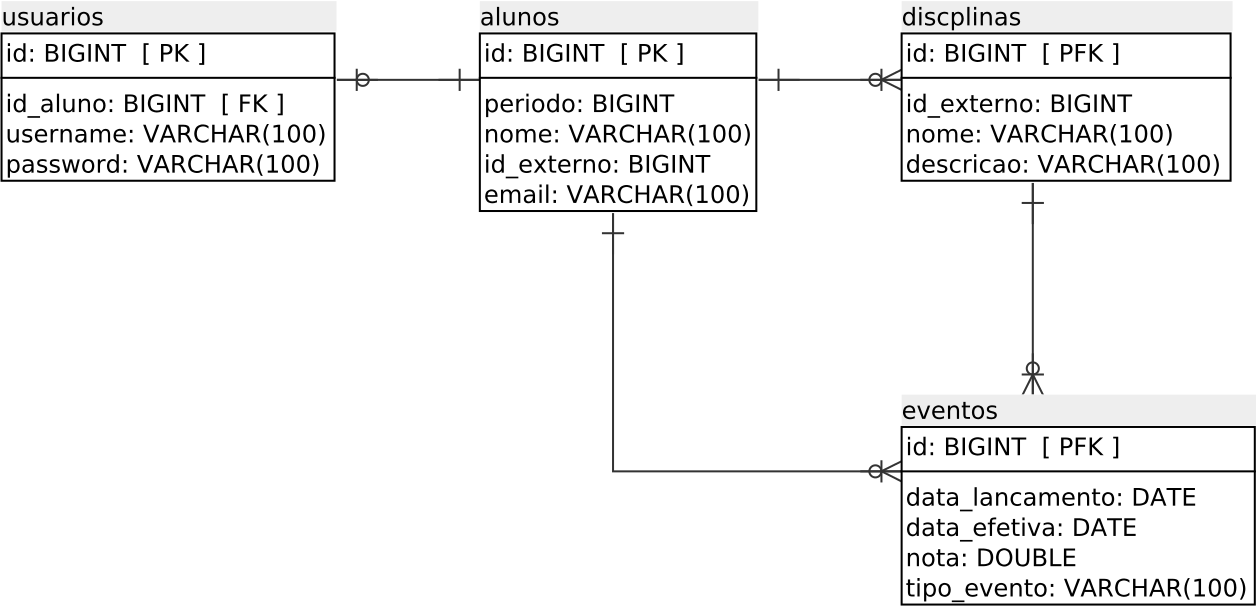
\includegraphics[scale=0.4]{./imagens/2_q_metodologico/qm9.png}}
			\caption[Diagrama de Entidade e Relacionamento]{Diagrama de Entidade e
			Relacionamento.
			\textbf{Fonte:}Elaborado pelos autores.}
			\label{fig:qm9}
		\end{figure}
\pagebreak
		\par Fazendo uso desse diagrama foi possível criar todas as classes 
	\textit{Java} que representam as entidades do mapeamento objeto-relacional. 
	Essas classes foram criadas fazendo uso de anotações próprias do
	\textit{Hibernate}, que é um \textit{framework} que implementa a especificação
	JPA\footnote{JPA - \textit{Java Persistense API}}. Essas classes fazem parte
	dos mecanismos de persistêcia de dados e são simplesmente t ou seja, objetos
	simples que contêm somente atributos privados e os métodos \textit{getters} e
	\textit{setters} que servem apenas para encapsular estes atributos. Uma das
	classes criadas, foi a classe \texttt{Aluno.java} que representa a tabela
	\texttt{alunos} no banco de dados e está representada na Figura
	\ref{fig:qm10}.%mudar para figura
	
		\begin{figure}[h!]
			\centerline{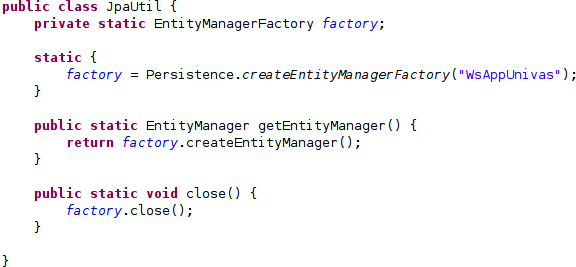
\includegraphics[scale=0.7]{./imagens/2_q_metodologico/qm10.png}}
			\caption[Classe \texttt{Aluno}]{Classe \texttt{Aluno}.
			\textbf{Fonte:}Elaborado pelos autores.}
			\label{fig:qm10} 
		\end{figure}
		
		\pagebreak
		
		\par Foram criadas outras classes \textit{Java} com a mesma finalidade da
	anterior, porém com pequenas diferenças no que diz respeito à atributos,
	metodos e anotações. Estas classes representam, de maneira individual, as
	tabelas no banco de dados. Certos atributos dessas classes têm por finalidade
	representar as colunas de cada tabela. Já os atributos que armazenam instâncias
	de outras classes ou até mesmo conjuntos (coleções) de instâncias representam os
	relacionamentos entre as tabelas. E por fim, para cada classe que representa uma
	entidade, foi necessário implementar os métodos \texttt{hashCode} e
	\texttt{equals}, para que estas pudessem facilmente ser comparadas e
	diferenciadas em relação aos seus valores, haja visto que cada instância
	destas classes representa um registro no banco de dados.
		
		\par Em seguida à criação das entidades, foi necessário configurar o arquivo
	\texttt{persistence.xml} que fica dentro do \textit{classpath} do projeto
	\textit{Java} ou seja, dentro da mesma pasta onde estão contidos pacotes do
	projeto. Este arquivo é extremamente importante, pois é nele que estão todas
	as configurações relativas à conexão com o banco de dados, configurações
	referentes ao Dialeto SQL que vai ser usado para as consultas e configurações
	referentes ao \textit{persistence unit} que é o conjunto de classes mapeadas
	para o banco de dados.	O arquivo \texttt{persistence.xml} está exposto no
	código \ref{fig:qm11}.
	
 		\begin{figure}[h!]
			\centerline{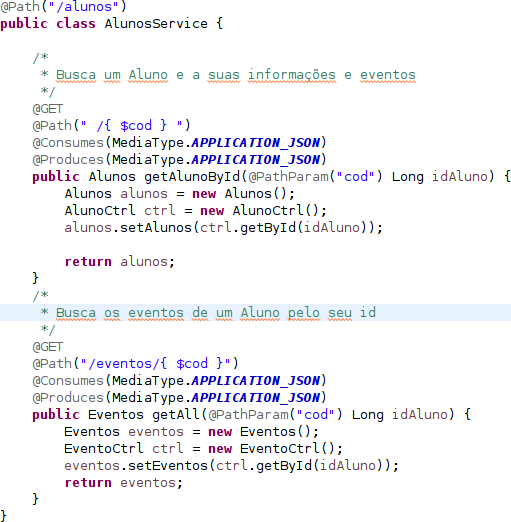
\includegraphics[scale=0.6]{./imagens/2_q_metodologico/qm11.png}}
			\caption[Arquivo \texttt{persistence.xml}]{Arquivo \texttt{persistence.xml}.
			\textbf{Fonte:}Elaborado pelos autores.}
			\label{fig:qm11}
		\end{figure}
		
			\par Em seguida à confecção do \texttt{persistence.xml} foi criada a
		classe \texttt{JpaUtil} que está representada na Figura \ref{fig:qm12}.
		Esta classe é responsável por criar uma \texttt{EntityManagerFactory} que é
		uma  fábrica de instâncias de \texttt{EntityManager} que nada mais é que um
		\textit{persistence unit} ou unidade de persistência. Essa classe tem a
		responsabilidade de prover um modo de comunicação entre a aplicação e o banco
		de dados. No entanto a classe \texttt{JpaUtil} cria uma única instância de
		\texttt{EntityManagerFactory}, que é responsável por disponibilizar e
		gerenciar as instâncias de \texttt{EntityManager} de acordo com a necessidade
		da aplicação.
		
		\pagebreak
		\begin{figure}[h!]
			\centerline{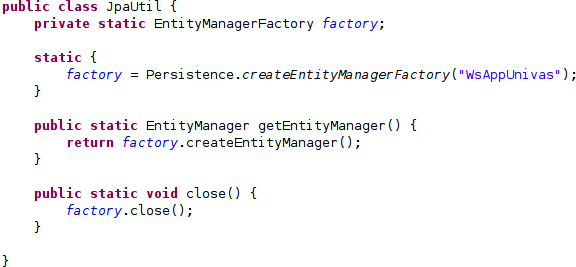
\includegraphics[scale=0.7]{./imagens/2_q_metodologico/qm12.png}}
			\caption[Classe \texttt{JpaUtil}]{Classe \texttt{JpaUtil}.
			\textbf{Fonte:}Elaborado pelos autores.}
			\label{fig:qm12}
		\end{figure}
		
	\par Em seguida à construção das classes que fazem a parte da persistência de
dados, foi desenvolvido a parte de disponibilização de serviços
\textit{RESTful}, fazendo uso do \textit{framework} \textit{Jersey}. Com isso
pode-se construir a classe que representa o primeiro serviço do
\textit{webservice}, que é a classe \texttt{Alunos}. Essa classe representa um
contexto REST, e portanto, dispõe de alguns recursos. Esses recursos fazem a
recuperação e a transmissão dos dados do \textit{webservice} para o aplicativo
\textit{Android}. Essa classe e seus respectivos métodos  estão representada na
Figura \ref{fig:qm13}.

		\begin{figure}[h!]
			\centerline{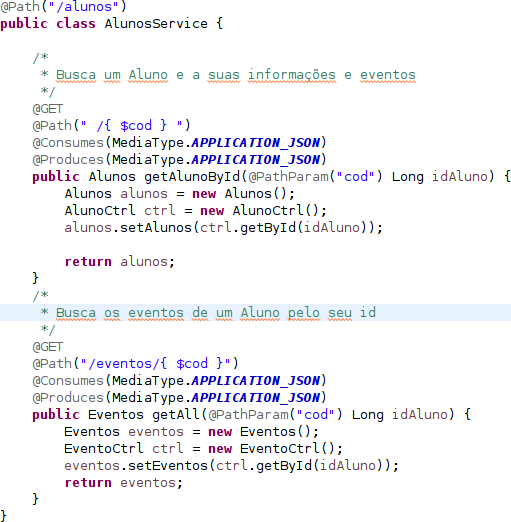
\includegraphics[scale=0.7]{./imagens/2_q_metodologico/qm13.png}}
			\caption[Classe \texttt{AlunosService}]{Classe \texttt{AlunosService}.
			\textbf{Fonte:}Elaborado pelos autores.}
			\label{fig:qm13}
		\end{figure}
		
		\par O \textit{webservice} pode fazer a busca de alunos pelo \texttt{id}
passado ou retornar uma coleção de eventos vinculados a um alunos, dependendo
do recurso acessado. Os tipos de dados que o \textit{webservice} consome e
retorna é o JSON\footnote{JSON - \textit{Javascript Object Notation}}. Não foi
necessário fazer nenhuma implementação adicional relativa a este formato, pois
o próprio \textit{framework Jersey} faz o tratamento e a conversão dos tipos de
entrada e saída de dados. No caso do saída de dados, faz a conversão de objetos 
\textit{Java} para JSON. E no caso de entrada tranforma um JSON em objeto
\textit{Java} já conhecido pelo \textit{webservice}. Com isso concluiu-se o
desenvolvimento do \textit{webservice} que fornece os dados para o aplicativo.

	\par Para que fosse possível transmitir dados para o aplicativo, era
necessário receber as informações do sistema acadêmico da referida instituição,
haja vista que o \textit{web service} é independente do mesmo. Para esse
propósito é necessário  contruir um módulo que faça a importação dos dados
necessários para a base de dados do \textit{web service}. Este por sua vez
terá a responsabilidade de fazer a importação dos dados periodicamente, e
ainda tratar os tipos de dados recebidos para tipos aplicáveis ao banco de
dados local. Além disso é preciso notificar o módulo responsável por invocar
o serviço \textit{Google Cloud Messaging} para que os dispositivos dos alunos
aos quais houveram atualizações nos dados, fossem notificados e fizessem acesso
ao \textit{web service} para solicitar esses dados atualizados.

	\par Os procedimentos acima citados foram os passos até agora realizados com o
propósito de se alcançar os resultados esperados para essa pesquisa.
	
						%Ambiente de desenvolvimento
						\subsubsection{Montagem do Ambiente de Desenvolvimento}
							%\subsubsection{Montagem do Ambiente de Desenvolvimento}
	
	\par No que diz respeito à contrução do \textit{web service}, foi necessária a
instalação e configuração de um ambiente de desenvolvimento compatível com as
necessidades apresentadas pelo software.

	\par A princípio foi instalado o \textit{Servlet Container} Apache Tomcat em
sua versão de número {7}. Este \textit{Servlet Container} foi instalado pois
implementa a API da especificação \textit{Servlets} {3.0} do Java. Isso era
necessário pelo fato que o \textit{framework} Jersey usa \textit{servlets} para
disponibilizar serviços REST. Além disso o Apache Tomcat foi escolhido, para
que o \textit{web service} pudesse fornecer os serviços necessários para o
consumo do aplicativo, na arquitetura REST, que sugere o uso do protocolo
HTTP\footnote{HTTP - Hypertext Transfer Protocol} para troca de mensagens, pois
além da funcionalidade com \textit{Servlets}, o Apache Tomcat também é um
servidor HTTP.
	
	\par O Apache Tomcat foi instalado, por meio do \textit{download} de um
arquivo compactado, de seu site oficial. A instalação consiste apenas
em extrair os dados do arquivo em uma pasta da preferência do desenvolvedor.
Esta abordagem permitiu a integração do Apache Tomcat com a
IDE\footnote{IDE - Integrated Development Environment}
Eclipse, que foi usada para o desenvolvimento. Com isto foi possível controlar
e monitorar, o servidor de aplicações através da IDE. Além da configuração
necessária para integrar o servidor à IDE, nenhuma outra configuração foi
necessária.

	\par Como ferramenta para desenvolvimento, foi usada a IDE Eclipse na versão
{4.4}, que é popularmente conhecida como Luna. O processo de instalação e
configuração da IDE, se assemelha bastante ao processo de instalação do Apache
Tomcat, pois somente é necessário fazer o download do arquivo compactado que é
fornecido na página do projeto, e descompactá-lo no local preferido pelo
desenvolvedor.

	\par Para armazenar os dados gerados e/ou recebidos, foi necessário fazer a
intalação do Sistema Gerenciador de Banco de Dados (SGBD) PostGreSql na sua
versão de número {9.4}. Como está sendo usado um sistema operacional baseado em
GNU/Linux como ambiente de desenvolvimento, o PostGreSql foi instalado através
do gerenciador de pacotes da distribuição.
 
%	\par Foi necessário criar um usuário no SGDB que tivesse permissão suficiente
%apenas para fazer as operações referentes ao banco de dados do \textit{web
%service}, evitando assim a necessidade de se trabalhar diretamente com um
%usuário master do SGBD. Esta medida foi tomada visando a segurança do banco de
%dados, pois com isto foi possível isolar e restringir as responsabilidades
% deste usuário.

	
						%desenvolvimento
						\subsubsection{Desenvolvimento}
							%\subsubsection{Desenvolvimento}

	%01 - Criação do database
	
	\par Com o ambiente de desenvolvimento pronto, começou de fato o
desenvolvimento. Primeiramente foi necessário criar o banco de dados no SGDB.
Este por sua vez foi criado com a ajuda do PgAdmin que é um software gráfico
para administração do SGDB, e que fornece uma interface gráfica de apoio para o
PotgreSql. Para criar era necessário ja estar com o PgAdmin aberto e conectado
a um servidor de banco de dados que neste caso era em servidor local como pode
ser visto na Figura \ref{fig:desws}.

	\begin{figure}[h!]
		\centerline{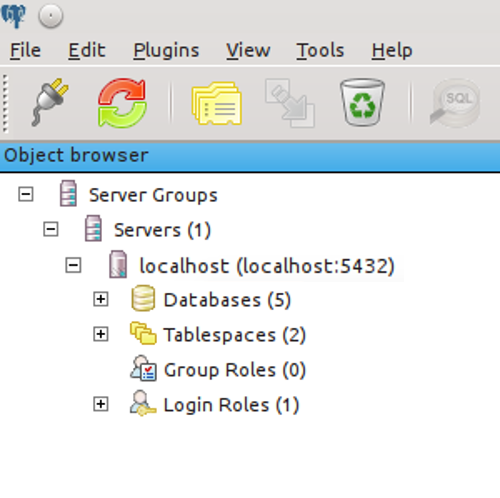
\includegraphics[scale=1]{./imagens/2_q_metodologico/4_procedimentos_resultados/43_webservice/432_desenvolvimento/desws.png}}
		\caption[Servidor de banco de dados local no PgAdmin]{Servidor de banco de
		dados local no PgAdmin.
			\textbf{Fonte:}Elaborado pelos autores.}
		\label{fig:desws}
	\end{figure}
	
	\pagebreak
	
	\par Para a efetiva criação do banco de dados era necessário clicar com o
botão direito do \textit{mouse}, sobre a opção \textbf{Databases -> New
Database\ldots} no PgAdmin, apresentada na Figura \ref{fig:desws1}.

	\begin{figure}[h!]
		\centerline{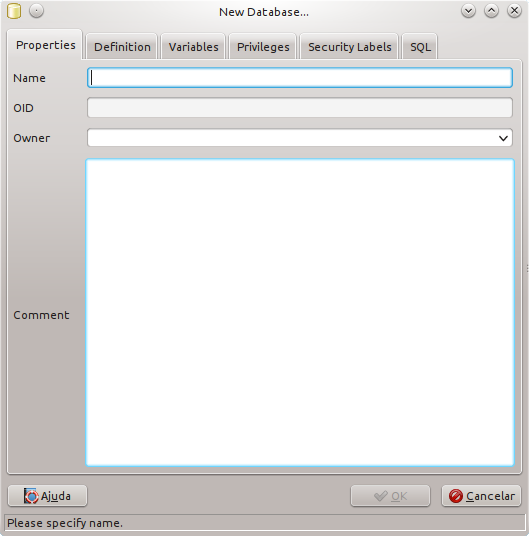
\includegraphics[scale=0.8]{./imagens/2_q_metodologico/4_procedimentos_resultados/43_webservice/432_desenvolvimento/desws1.png}}
		\caption[Opção \textit{New Database\ldots}]{Opção \textit{New Database\ldots}.
			\textbf{Fonte:}Elaborado pelos autores.}
		\label{fig:desws1}
	\end{figure}

	\pagebreak
	
	\par Em seguida foi necessário preencher o dados da janela apresentada, como
está apresentado na Figura \ref{fig:desws2}.
	
	\begin{figure}[h!]
		\centerline{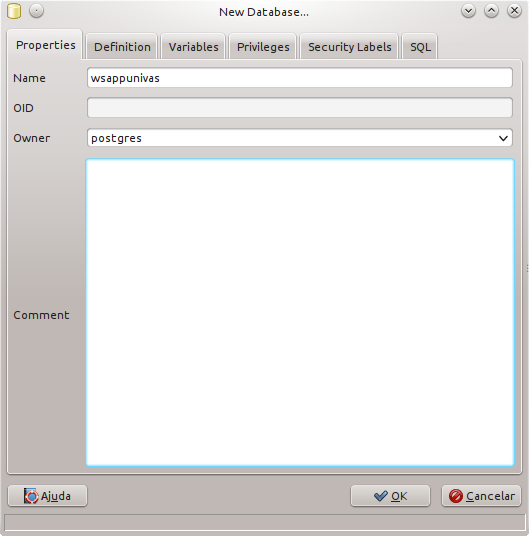
\includegraphics[scale=1]{./imagens/2_q_metodologico/4_procedimentos_resultados/43_webservice/432_desenvolvimento/desws2.png}}
		\caption[Tela \textit{New Database\ldots}]{Tela \textit{New Database\ldots}.
			\textbf{Fonte:}Elaborado pelos autores.}
		\label{fig:desws2}
	\end{figure}
	
	\pagebreak

	\par Como pode ser visto foram preenchidos os campos nome e usuário . O campo
nome se refere ao nome do banco de dados que foi definido com
\texttt{wsappunivas}, e usuário, o responsável pelo banco de dados, que para
este caso foi usuário padrão do SGDB, que é o \texttt{postgres}. Além destas
configurações mais nenhuma foi necessária. O banco de dados foi criado, porém
sua estrutura não foi definida, pois como será visto mais adiante o Hibernate,
possui um mecanismo, que com algumas configurações, permite a estruturação do
banco de dados, de acordo com o mapeamento objeto-relacional e de acordo com a
evolução do projeto. Isto permitirá mudanças na estrutura do banco de dados e
suas tabelas, e até mesmo eventuais correções.
	
	%02 - Início do projeto web no eclipse;
	\par Em seguida foi criado um projeto do tipo Dynamic Web Project no
Eclipse. Para proceder com a criação de um novo projeto deste tipo no Eclipse, é
necessário acessar na IDE, a opção \textbf{File -> New-> Dynamic Web Project}
como pode ser visto na figura \ref{fig:desws3}.

	
	\begin{figure}[h!]
		\centerline{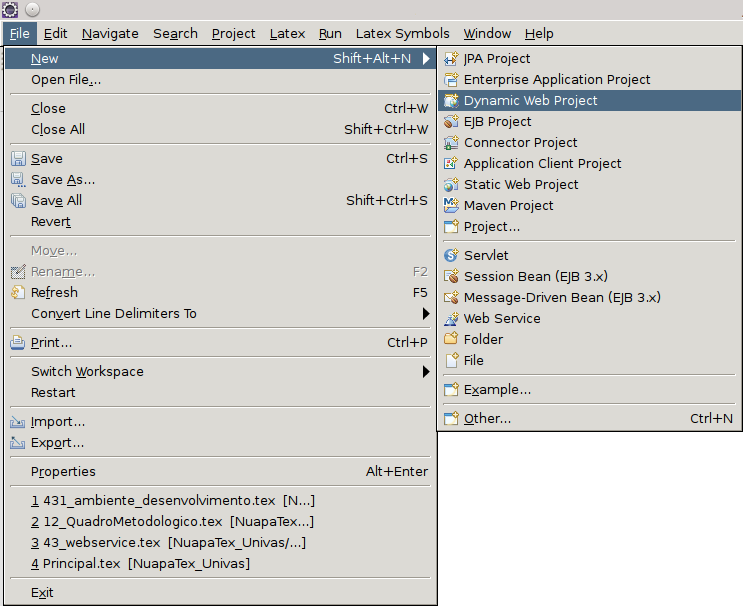
\includegraphics[scale=0.8]{./imagens/2_q_metodologico/4_procedimentos_resultados/43_webservice/432_desenvolvimento/desws3.png}}
		\caption[Tela \textit{New Database\ldots}]{Tela \textit{New Database\ldots}.
			\textbf{Fonte:}Elaborado pelos autores.}
		\label{fig:desws3}
	\end{figure}
	
	\pagebreak
	
 	\par Em seguida foi apresentada uma tela para o preenchimento de alguns dados
 requeridos para a criação do projeto. Destas informações somente foi preenchido
 o nome do projeto. As outras informações continuaram sendo as que vem por
 padrão da IDE. A janela apresentada e as informações preenchidas podem ser
 vistas na Figura \ref{fig:desws4}.

	\begin{figure}[h!]
		\centerline{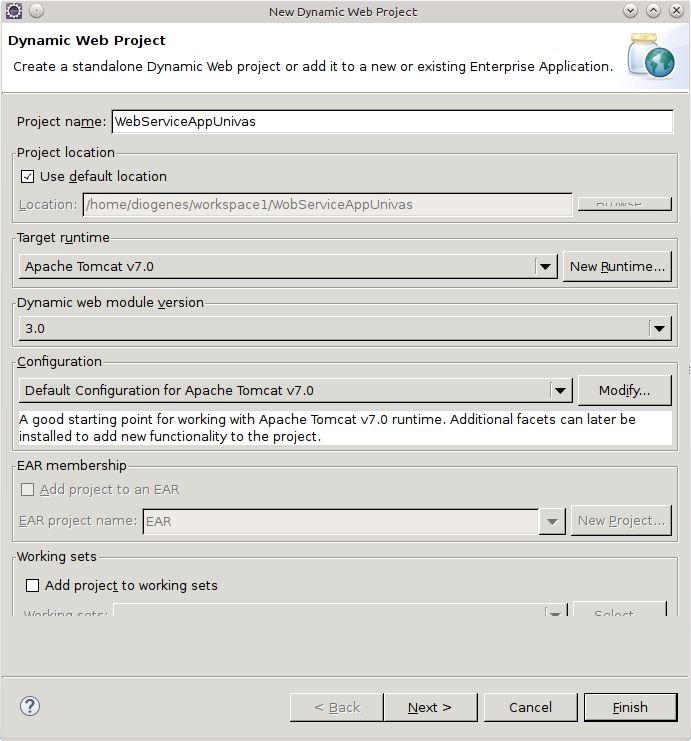
\includegraphics[scale=0.8]{./imagens/2_q_metodologico/4_procedimentos_resultados/43_webservice/432_desenvolvimento/desws4.png}}
		\caption[Tela para criação de um novo projeto no Eclipse]{Tela para criação de um novo projeto no Eclipse.
			\textbf{Fonte:}Elaborado pelos autores.}
		\label{fig:desws4}
	\end{figure}
	
	\pagebreak
	
	
	\par Na próxima janela apresentada, que têm por função configurar a pasta de
códigos do projeto manteve-se a configuração apresentada pela IDE, como mostra
a Figura \ref{fig:desws5}.

	\begin{figure}[h!]
		\centerline{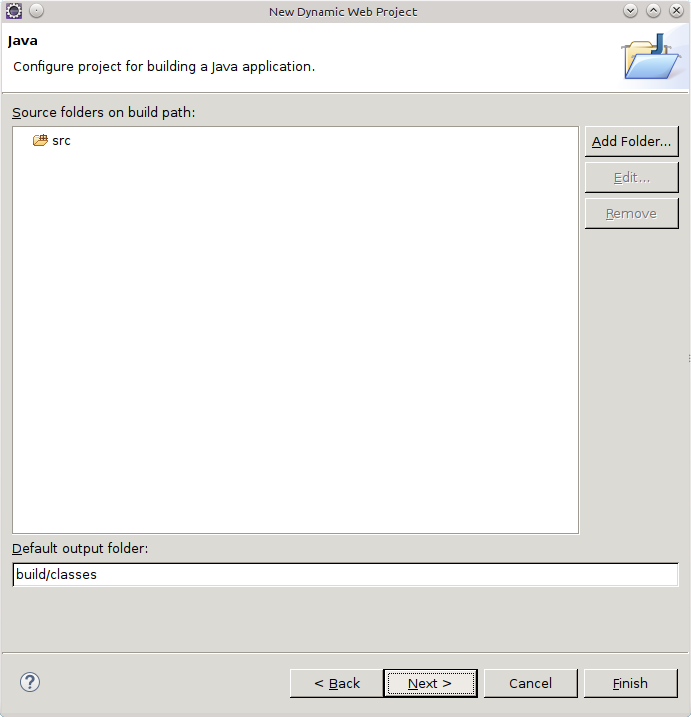
\includegraphics[scale=0.8]{./imagens/2_q_metodologico/4_procedimentos_resultados/43_webservice/432_desenvolvimento/desws5.png}}
		\caption[Tela para criação de um novo projeto no Eclipse]{Tela para criação de um novo projeto no Eclipse.
			\textbf{Fonte:}Elaborado pelos autores.}
		\label{fig:desws5}
	\end{figure}
	
	\pagebreak
	
	\par Na sequencia, na tela que foi apresentada era necessário preencher o
campo \textbf{Context root:} com o contexto principal da aplicação web que
acabou mantendo o próprio nome da aplicação. Além disso foi marcado a opção
\textbf{Generate web.xml deployment descriptor}, para que ao criar o projeto, a
própria IDE criasse o arquivo \texttt{web.xml}, arquivo responsável por algumas
configurações da aplicação web. Esta tela esta apresentada na Figura
\ref{fig:desws6}.

	\begin{figure}[h!]
		\centerline{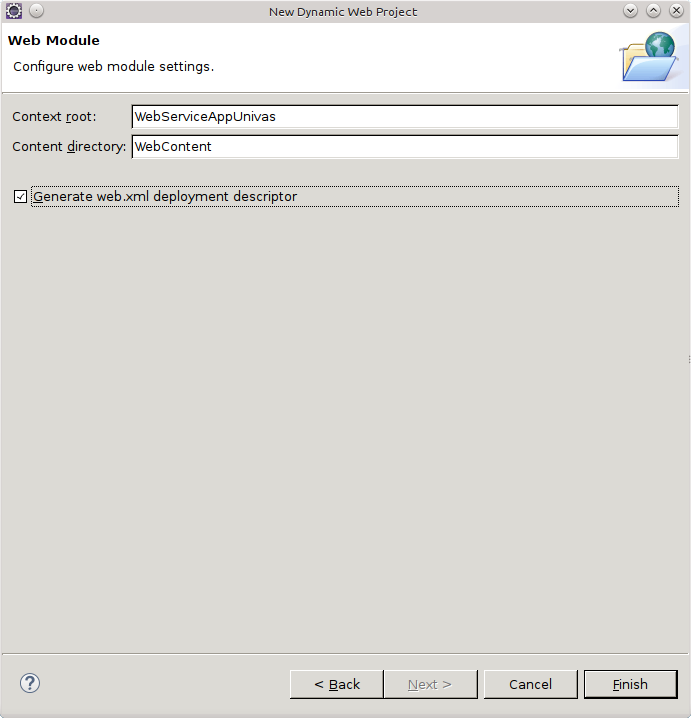
\includegraphics[scale=0.8]{./imagens/2_q_metodologico/4_procedimentos_resultados/43_webservice/432_desenvolvimento/desws6.png}}
		\caption[Tela para criação de um novo projeto no Eclipse]{Tela para criação de um novo projeto no Eclipse.
			\textbf{Fonte:}Elaborado pelos autores.}
		\label{fig:desws6}
	\end{figure}
	
	\pagebreak

	%03 - Mapeamento orm;	
		%	->Criação do pacote

	\par Após este passo foi concluído a criação do projeto, e já era possível
iniciar os trabalhos com a camada de persistência de dados do projeto. Para
este propósito, primeiramente foi criado um pacote, onde ficaram contidas as
classes que representam as entidades do ORM. Para a criação do pacote foi
necessário clicar com o botão direito do mouse sobre o projeto e acessar a opção
\textbf{New -> Package}, como pode ser visto na Figura \ref{fig:desws7}.

	\begin{figure}[h!]
		\centerline{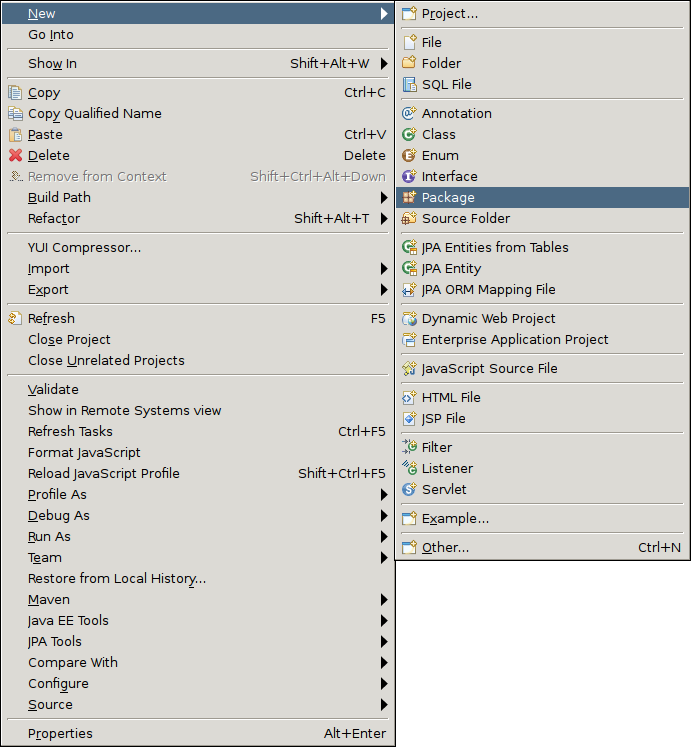
\includegraphics[scale=0.8]{./imagens/2_q_metodologico/4_procedimentos_resultados/43_webservice/432_desenvolvimento/desws7.png}}
		\caption[Tela para criação de um novo projeto no Eclipse]{Tela para criação de um novo projeto no Eclipse.
			\textbf{Fonte:}Elaborado pelos autores.}
		\label{fig:desws7}
	\end{figure}
	
	\pagebreak 
	
	\par Em seguida foi apresentada a janela New Java Package, para a criação de
um novo pacote mostrada na Figura \ref{fig:desws8}. O pacote recebeu o nome de
"\texttt{br.edu.univas.restapiappunivas.model}", pois nele estão contidas as
classes que fazem parte do modelo de negócios da aplicação. Este pacote foi
criado visando a divisão das responsabilidades internas no projeto, além de
contribuir positivamente com a organização do mesmo.

	\begin{figure}[h!]
		\centerline{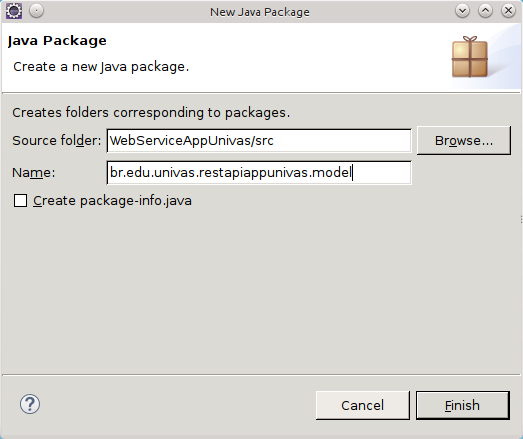
\includegraphics[scale=0.8]{./imagens/2_q_metodologico/4_procedimentos_resultados/43_webservice/432_desenvolvimento/desws8.png}}
		\caption[Tela para criação de um novo projeto no Eclipse]{Tela para criação de um novo projeto no Eclipse.
			\textbf{Fonte:}Elaborado pelos autores.}
		\label{fig:desws8}
	\end{figure}
	
	\pagebreak
		
		%	->Criação das classes
	\par Com este pacote criado, ja era possível criar as classes do ORM. Foi
criada primeiramente a classe \texttt{Student.java}. Para a criação desta classe
foi necesário clicar com o botão direito do \textit{mouse} sobre o projeto e
navegar até a opção \textbf{New -> Class} como pode ser visto na Figura
\ref{fig:desws9}. 

	\begin{figure}[h!]
		\centerline{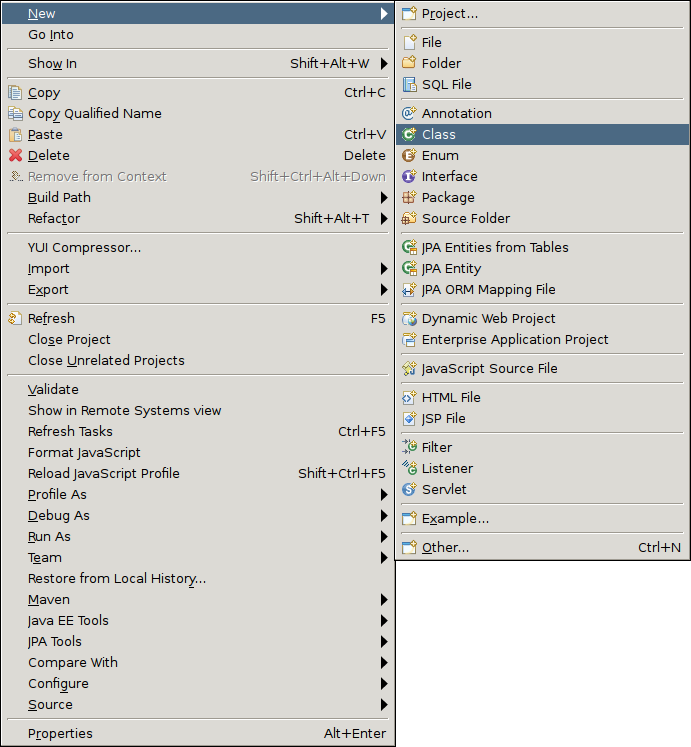
\includegraphics[scale=0.8]{./imagens/2_q_metodologico/4_procedimentos_resultados/43_webservice/432_desenvolvimento/desws9.png}}
		\caption[Sem legenda]{Sem legenda.
			\textbf{Fonte:}Elaborado pelos autores.}
		\label{fig:desws9}
	\end{figure}
	
	\pagebreak


	\par Em seguida foi apresentada uma janela chamada New Java Class. Nesta
janela somente foi necessário preencher o campo \textbf{Name:} que representa o
nome da classe que está sendo criada.
	
	
	
	 \begin{figure}[h!]
		\centerline{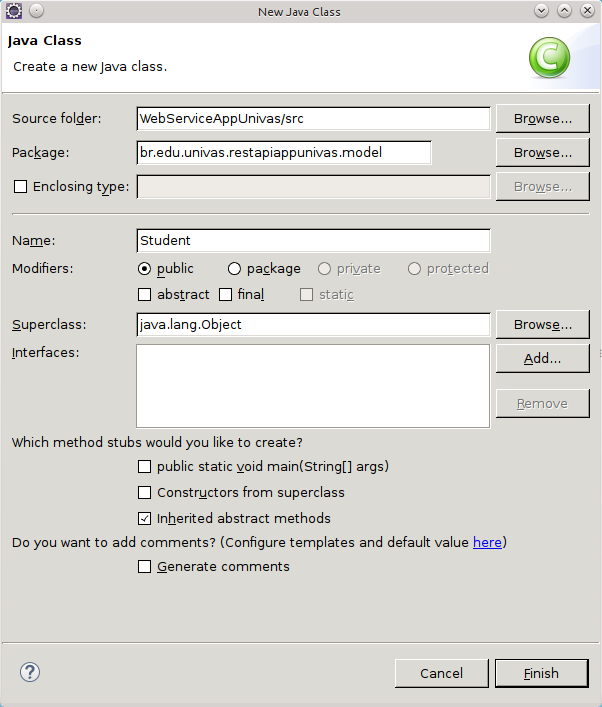
\includegraphics[scale=0.8]{./imagens/2_q_metodologico/4_procedimentos_resultados/43_webservice/432_desenvolvimento/desws10.png}}
		\caption[Sem legenda]{Sem legenda.
			\textbf{Fonte:}Elaborado pelos autores.}
		\label{fig:desws10}
	\end{figure}
	
	\pagebreak

	\par Esta classe foi definida para representar as informações referente aos
alunos. o código da classe pode ser visto na Figura \ref{fig:desws11}. 
	
	
	\begin{figure}[h!]
		\begin{lstlisting} [style=custom_Java]	
	package br.edu.univas.restapiappunivas.model;
	/**
	 *imports omitidos
	 */
	
	@Entity
	@Table(name = "student")
	public class Student {
	
		@Id
		@SequenceGenerator(name = "id_student", sequenceName = "seq_id_student",
			allocationSize = 1) 
		@GeneratedValue(generator = "id_student", strategy = GenerationType.IDENTITY)
		@Column(name = "id_student", nullable = false)
		private Long idStudent;
	
		@Column(name = "id_external", nullable = false)
		private Long idDatabaseExternal;
	
		@Column(length = 100, nullable = false)
		private String name;
	
		@Column(length = 100, nullable = false)
		private String email;
	
		@OneToMany(mappedBy="student", fetch = FetchType.EAGER)
		private List<Event> events;
	
		@OneToOne(optional = false, fetch = FetchType.LAZY)
		@JoinColumn(name = "id_user")
		private User user;
	
		/**
		 * Omitidos todos Getters e Setters
		 */
	
		@Override
		public int hashCode() {
			/**
			 * Omitido
			 */
		}
	
		@Override
		public boolean equals(Object obj) {
			/**
			 * Omitido
			 */
		}
	
	}
\end{lstlisting}
		\caption[Sem legenda]{Sem legenda.
			\textbf{Fonte:}Elaborado pelos autores.}
		\label{fig:desws11}
	\end{figure}
	
	\pagebreak
	
	\par É válido lembrar esta classe possui anotações para que possa ser
reconhecida como uma entidade do JPA, e assim persistida no banco de dados
quando necessário. Além disso estas anotações possuem outras finalidades
específicas. A seguir estão listadas todas as anotações  que foram usadas na
classe \texttt{Student.java} e nas outras classes que fazem parte do mapeamento
objeto relacional da aplicação.

	\begin{itemize}
	  \item \texttt{@Entity}: esta anotação foi necessária para que esta classe
	  pudesse ser reconhecida como uma entidade do JPA e assim persistida no banco
	  de dados;
	  \item \texttt{@Table}: anotação que possui algumas configurações relativas a
	  tabela no banco de dados, a qual esta entidade representa, no caso da classe'
	  mostrada anteriormente é configurado o nome da tabela;
	  \item \texttt{@Id}: esta anotação fica sobre o atributo que representa a
	  chave primária no banco de dados;
	  \item \texttt{@SequenceGenerator}: esta anotação define qual será o modo com
	  que a chave primaria será incrementada.
	  \item \texttt{@Column}: define algumas propriedades do campo da tabela do
	  banco de dados, o qual o atributo que ele anota representa. Estas
	  configuraçãoes podem são:
		  	\begin{itemize}
		    	\item \texttt{name}: muda o nome do campo;
		    	\item \texttt{length}: determina o tamanho em caracteres que o campo
		    	aceitará;
		    	\item \texttt{nullable}: define se o preenchimento do campo é obrigatório;
		    	\item \texttt{unique}: este atributo define se o campo aceitará valores
		    	únicos;
		    \end{itemize}
	  \item \texttt{@OneToMany}: representa um relacionamento um-para-muitos no
	  banco de dados. Anotam coleções de outras entidades;
	  \item \texttt{@ManyToOne}: representa um relacionamento
	  muitos-para-um no banco de dados. Este é a contraparte da anotação
	  um-para-muitos;
	  \item \texttt{@OneToOne}: representa um relacionamento um-para-um no banco de
	  dados.
\end{itemize}
 
	\par Esta classe faz parte do mecanismo de persistêcia de dados e é
simplesmente um  pojo ou seja, um objeto  simples que contêm somente atributos
privados e os métodos \textit{getters} e \textit{setters} que servem apenas
para encapsular estes atributos. Além desta classe, foram criadas outras com os
mesmos propósitos. Estas classes podem ser vistas na Figura \ref{fig:desws12}. 
	
	
	\begin{figure}[h!]
		\centerline{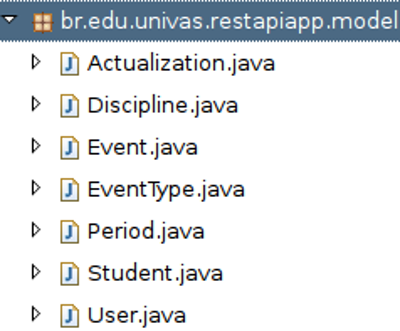
\includegraphics[scale=0.8]{./imagens/2_q_metodologico/4_procedimentos_resultados/43_webservice/432_desenvolvimento/desws12.png}}
		\caption[Sem legenda]{Sem legenda.
			\textbf{Fonte:}Elaborado pelos autores.}
		\label{fig:desws12}
	\end{figure}
	
	\pagebreak
	
	\par Estas classes tinham a mesma finalidade da anterior, porém com pequenas
diferenças no que diz respeito à atributos, metodos e anotações. Estas classes
representam, de maneira individual, as tabelas no banco de dados.

	%04 - HashCode e equals
	\par E por fim, para cada classe que representa uma entidade, foi necessário
implementar os métodos \texttt{hashCode} e \texttt{equals}, para que estas
pudessem facilmente ser comparadas e diferenciadas em relação aos seus
valores, haja visto que cada instância destas classes representa um registro
no banco de dados.
	
	%05 - Configuração do persistence.xml
	\par Em seguida à criação das entidades, foi necessário configurar o arquivo
\texttt{persistence.xml} que fica dentro do \textit{classpath} do projeto
Java ou seja, dentro da mesma pasta onde estão contidos pacotes do
projeto. Este arquivo é extremamente importante, pois é nele que estão todas
as configurações relativas à conexão com o banco de dados, configurações
referentes ao Dialeto SQL que vai ser usado para as consultas e configurações
referentes ao \textit{persistence unit} que é o conjunto de classes mapeadas
para o banco de dados.	O arquivo \texttt{persistence.xml} está exposto na
Figura \ref{fig:qm11}.

	\begin{figure}[h!]
		%persistence.xml
\begin{lstlisting} [style=custom_XML]
<?xml version="1.0" encoding="UTF-8"?>
<persistence version="2.1"
	xmlns="http://xmlns.jcp.org/xml/ns/persistence" 
	xmlns:xsi="http://www.w3.org/2001/XMLSchema-instance"
	xsi:schemaLocation="http://xmlns.jcp.org/xml/ns/persistence
	http://xmlns.jcp.org/xml/ns/persistence/persistence_2_1.xsd">
		<persistence-unit name="WsAppUnivas" transaction-type="RESOURCE_LOCAL">
					<provider>
						org.hibernate.jpa.HibernatePersistenceProvider
					</provider>
					<properties>
								<property name="javax.persistence.jdbc.url"
									value="jdbc:postgresql://localhost:5432/wsappunivas" />
								<property name="javax.persistence.jdbc.user" 
									value="postgres" />
								<property name="javax.persistence.jdbc.password" 
									value="omitido" />
								<property name="javax.persistence.jdbc.driver" 
									value="org.postgresql.Driver" />
								<property name="hibernate.dialect" 
									value="org.hibernate.dialect.PostgreSQLDialect" />
								<property name="hibernate.format_sql" 
									value="true" />
								<property name="hibernate.temp.use_jdbc_metadata_defaults"
									value="false" />
								<property name="hibernate.show_sql" 
									value="true" />
								<property name="hibernate.hbm2ddl.auto" 
									value="create" />
					</properties>
		</persistence-unit>
</persistence>
\end{lstlisting}
		\caption[Arquivo \texttt{persistence.xml}]{Arquivo \texttt{persistence.xml}.
		\textbf{Fonte:}Elaborado pelos autores.}
		\label{fig:qm11}
	\end{figure}
	
	%06 - Confecção JpaUtil.java
	\par Em seguida à confecção do \texttt{persistence.xml} foi criada a
classe \texttt{JpaUtil} que está representada na Figura \ref{fig:qm12}.
Esta classe é responsável por criar uma \texttt{EntityManagerFactory} que é
uma  fábrica de instâncias de \texttt{EntityManager} que nada mais é que um
\textit{persistence unit} ou unidade de persistência. Essa classe tem a
responsabilidade de prover um modo de comunicação entre a aplicação e o banco
de dados. No entanto a classe \texttt{JpaUtil} cria uma única instância de
\texttt{EntityManagerFactory}, que é responsável por disponibilizar e
gerenciar as instâncias de \texttt{EntityManager} de acordo com a necessidade
da aplicação.
	
	\pagebreak
	\begin{figure}[h!]
		%classe JpaUtil.java

\begin{lstlisting} [style=custom_Java] 	
package br.edu.univas.restapiappunivas.util;

import javax.persistence.EntityManager;
import javax.persistence.EntityManagerFactory;
import javax.persistence.Persistence;

public class JpaUtil {
	private static EntityManagerFactory factory;

	static {
		factory = Persistence.createEntityManagerFactory("WsAppUnivas");
	}

	public static EntityManager getEntityManager() {
		return factory.createEntityManager();
	}

	public static void close() {
		factory.close();
	}

}
	
\end{lstlisting}
		\caption[Classe \texttt{JpaUtil.java}]{Classe \texttt{JpaUtil.java}.
		\textbf{Fonte:}Elaborado pelos autores.}
		\label{fig:qm12}
	\end{figure}
		
	\par Em seguida à construção das classes que fazem a parte da persistência de
dados, foi desenvolvido a parte de disponibilização de serviços
RESTful, fazendo uso do \textit{framework} Jersey. Com isso
pode-se construir a classe que representa o primeiro serviço do
\textit{webservice}, que é a classe \texttt{Alunos}. Essa classe representa um
contexto REST, e portanto, dispõe de alguns recursos. Esses recursos fazem a
recuperação e a transmissão dos dados do \textit{web service} para o aplicativo
Android. Essa classe e seus respectivos métodos  estão representada na
Figura .
		
		\par O \textit{webservice} pode fazer a busca de alunos pelo \texttt{id}
passado ou retornar uma coleção de eventos vinculados a um alunos, dependendo
do recurso acessado. Os tipos de dados que o \textit{webservice} consome e
retorna é o JSON\footnote{JSON - Javascript Object Notation}. Não foi
necessário fazer nenhuma implementação adicional relativa a este formato, pois
o próprio \textit{framework} Jersey faz o tratamento e a conversão dos tipos de
entrada e saída de dados. No caso do saída de dados, faz a conversão de objetos 
Java para JSON. E no caso de entrada tranforma um JSON em objeto
Java já conhecido pelo \textit{web service}. Com isso concluiu-se o
desenvolvimento do \textit{web service} que fornece os dados para o aplicativo.

	%23 - Módulo que ira fazer a busca dos dados na base da instituição de ensino
	%24 - Falar que vai ser simulado
	\par Para que fosse possível transmitir dados para o aplicativo, era
necessário receber as informações do sistema acadêmico da referida instituição,
haja vista que o \textit{web service} é independente do mesmo. Para esse
propósito é necessário  contruir um módulo que faça a importação dos dados
necessários para a base de dados do \textit{web service}. 

	\par Este por sua vez terá a responsabilidade de fazer a importação dos dados
periodicamente, e ainda tratar os tipos de dados recebidos para tipos
aplicáveis ao banco de dados local. Além disso é preciso notificar o módulo
responsável por invocar o serviço Google Cloud Messaging para que os
dispositivos dos alunos aos quais houveram atualizações nos dados, fossem
notificados e fizessem acesso ao \textit{web service} para solicitar esses
dados atualizados.

	\par Os procedimentos acima citados foram os passos até agora realizados com o
propósito de se alcançar os resultados esperados para essa pesquisa.






%07 - Explicar anotações dos pojos
%08 - Finalizando camada de persistência
%09 - Camada de serviço
%10 - Classes que disponibilizam serviços anotações
%11 - Explicar as entities criadas para disponibilizar os dados
%12 - Ctrls que fazem a busca dos dados
%13 - Problema do erro 500
%14 - Provedor de arquivos e contexto
%15 - Em todos citar o pom.xml
%16 - Configuração do web.xml
%17 - Módulo de varredura de atualizações com timerTask
%18 - Módulo de alerta de provas agendas no dia da prova
%20 - Módulo para disparar as mensagens para o gcm
%21 - Serviço que faz o registro de sender_id
%22 - Mostrar a estrutura do empacotamento depois de finalizado
							%implantação
						%\subsubsection{Implantação}	
						%	%\subsubsection{Implantação}